\documentclass{article}
\usepackage[utf8]{inputenc}

%% Language and font encodings
\usepackage[english,italian]{babel} 
\usepackage[T1]{fontenc}

\usepackage{subfig}

\usepackage{listings}
\usepackage{xcolor}

\usepackage{colortbl}

\colorlet{punct}{red!60!black}
\definecolor{background}{HTML}{EEEEEE}
\definecolor{delim}{RGB}{20,105,176}
\colorlet{numb}{magenta!60!black}

\lstdefinelanguage{json}{
    basicstyle=\small\ttfamily,
    numbers=left,
    numberstyle=\scriptsize,
    stepnumber=1,
    numbersep=8pt,
    showstringspaces=false,
    breaklines=true,
    frame=lines,
    backgroundcolor=\color{background},
    literate=
     *{0}{{{\color{numb}0}}}{1}
      {1}{{{\color{numb}1}}}{1}
      {2}{{{\color{numb}2}}}{1}
      {3}{{{\color{numb}3}}}{1}
      {4}{{{\color{numb}4}}}{1}
      {5}{{{\color{numb}5}}}{1}
      {6}{{{\color{numb}6}}}{1}
      {7}{{{\color{numb}7}}}{1}
      {8}{{{\color{numb}8}}}{1}
      {9}{{{\color{numb}9}}}{1}
      {:}{{{\color{punct}{:}}}}{1}
      {,}{{{\color{punct}{,}}}}{1}
      {\{}{{{\color{delim}{\{}}}}{1}
      {\}}{{{\color{delim}{\}}}}}{1}
      {[}{{{\color{delim}{[}}}}{1}
      {]}{{{\color{delim}{]}}}}{1},
}

\usepackage{natbib}
\usepackage{graphicx}
\usepackage{imakeidx}
\makeindex


\title{Relazione Progetto IoT 
(Safe Lab)}
\author{
  Adamo Fapohunda\\
  \texttt{0000907136}
  \and
  Laura Bugo\\
  \texttt{0000907116}
}
\date{ }



\begin{document}

\maketitle

\section{Introduzione}


L'obiettivo del progetto è quello di realizzare un sistema per il monitoraggio di un ambiente basandosi su tecnologie IOT. In particolare vengono misurati i valori ambientali di un locale (temperatura, umidità e pressione) e il numero di persone che si trovano all'interno di esso. Ci si è posti come intento quello di implementare il sistema utilizzando sensori e schede di sviluppo a bassa potenza e basso costo.

Nella relazione che segue verranno descritti in maniera approfondita gli strumenti utilizzati (Sezione \ref{section:environment}), l'architettura del progetto (Sezione \ref{section:architettura}), l'implementazione svolta (Sezione \ref{section:implementazione}) e i risultati ottenuti (Sezione \ref{section:risultati}).


\section{Environment}
\label{section:environment}

\subsection{Hardware}

Per i due obiettivi del progetto, ossia contare il numero di persone all'interno della stanza e rilevare i parametri ambientali sono stati utilizzate due single-board microcontroller NodeMCU dotate di connettività WiFi.

Per la raccolta e visualizzazione dei dati è stato utilizzato un Raspberry Pi 3, un single-board computer dotato di cpu ARM a 64 bit corredato da un hard disk drive (HDD) esterno.

\subsection{Software}

\begin{itemize}
    \item Docker e Docker-compose \cite{docker}: utilizzato per distribuire il software in container isolati e che hanno la possibilità di comunicare tra loro;
    \item Mozilla WebThings Framework e Mozilla WebThings Gateway  \cite{mozillaiot}: utilizzato per risolvere il problema della findability delle Thing connesse alla rete locale. Inoltre è in grado di gestire automaticamente la riconnessione con i devices;
    \item InfluxDB 2.0 \cite{influx}: utilizzato come database per il salvataggio dei dati sotto forma di time series;
    \item Grafana \cite{grafana}; utilizzato per permettere una visualizzazione interattiva dei dati ottenuti;
    \item Telegram: utilizzato per notificare all'utente situazioni di alerting.
\end{itemize}

Linguaggi utilizzati:
\begin{itemize}
    \item Arduino language (C/C++): per la programmazione delle board NodeMCU;
    \item Javascript/Typescrit: per la costruzione dei servizi;
    \item Python: per lo studio e l'implementazione di metodologie di forecasting sui dati e la costruzione del servizio di forecasting;
    \item Bash scripting.
\end{itemize}

\section{Architettura}
\label{section:architettura}

\begin{figure} [!b]
    \centering
    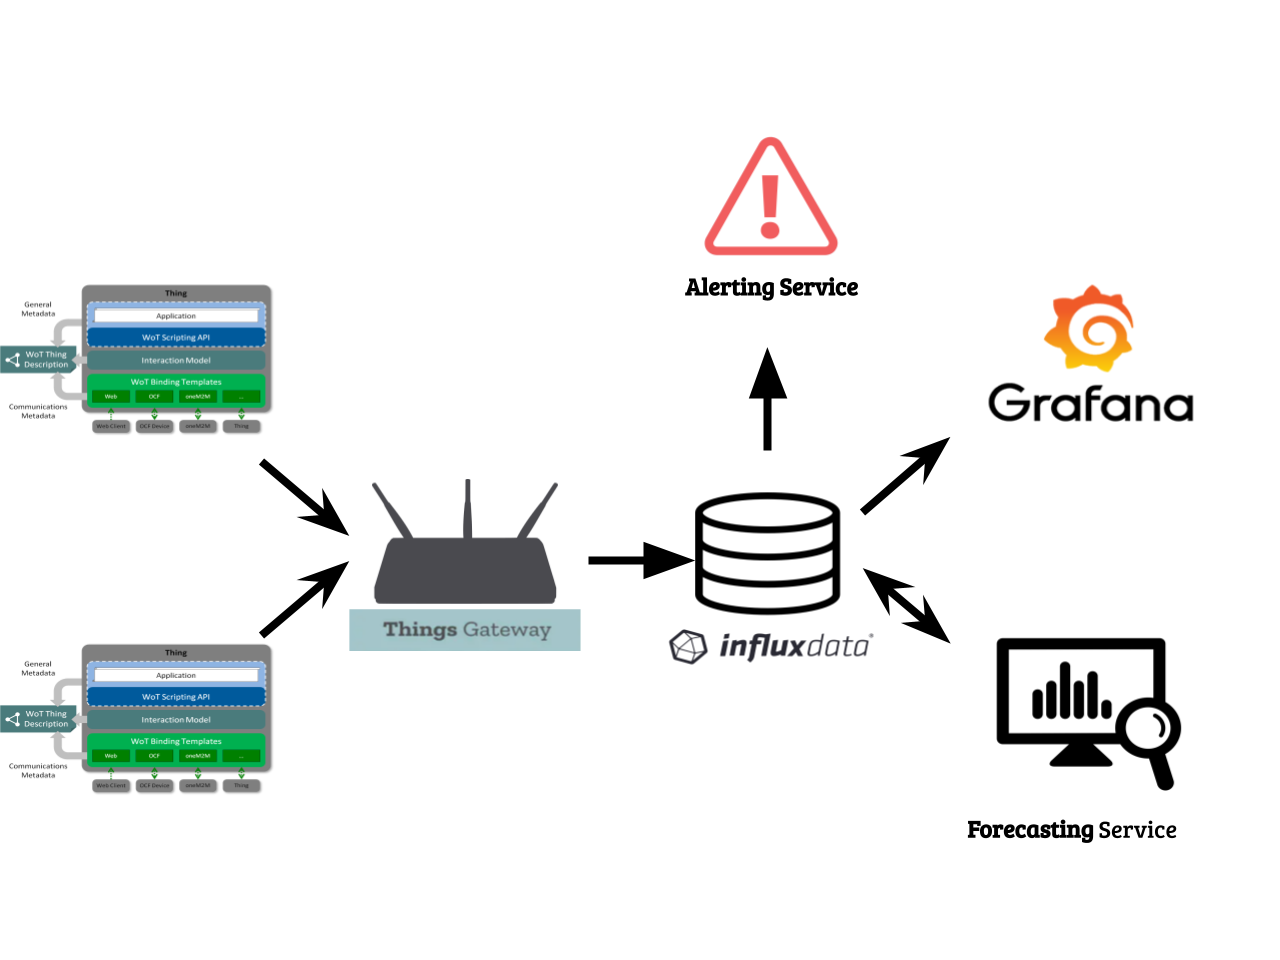
\includegraphics[width=12cm]{img/arch.png}
    \caption{Architettura}
    \label{fig:arch}
\end{figure}

Come è possibile osservare in Figura \ref{fig:arch}, sono stati costruiti due smart device che sono stati implementati come Web Things. Tali Thing sono rilevate dal  Gateway di Mozilla che funge da unico punto di accesso per caricare i dati su InfluxDB. I dati caricati su InfluxDB sono quindi analizzati per effettuare operazioni di forecasting sui livelli dei parametri ambientali e del numero di persone nell'ambiente. La visualizzazione dei dati è fornita attraverso le dashboard di Grafana. Inoltre è stato implementato un meccanismo di alerting per notificate l'utente attraverso Telegram nel caso in cui i parametri dell'ambiente raggiungano livelli critici.



\subsection{Docker}
Docker è stato utilizzato per poter mantenere i diversi servizi isolati tra loro, inoltre ci permette di garantire la riproducibilità degli ambienti di sviluppo. 
\medskip

Il container di Docker sono stati utilizzati per racchiudere i diversi servizi:
\begin{itemize}
    \item Mozilla Gateway;
    \item InfluxDB 2.0;
    \item Servizio di Forecasting:
    \begin{itemize}
        \item Writer Service;
        \item Forecasting Service.
    \end{itemize}
    \item Grafana;
    \item Servizio di alerting.
\end{itemize}
Tali container sono stati caricati su Raspberry Pi. Uno script di installazione permette di fare build delle immagini necessarie e gestire i servizi tramite Docker Compose. Tuttavia è necessario procurarsi i token di:
\begin{itemize}
    \item Mozilla Gateway;
    \item InfluxDB;
    \item Telegram.
\end{itemize}

\subsubsection{Problematiche riscontrate}

Dato che Influx non è disponibile per architetture ARM32, per poterlo installare nel Raspberry è stato necessario installare un sistema operativo a 64 bit, in particolare Ubuntu Server 20.04. In un secondo momento è stata creata un'immagine Docker ad hoc sfruttando la release a 64 bit, tuttavia la scelta di passare a un sistema operativo a 64 bit ha comportato a difficoltà dovute a incompatibilità tra TensorFlow e architetture ARM a 64 bit. 


\section{Implementazione}
\label{section:implementazione}
\subsection{Smart Things e WoT Things}
Nelle sezioni a seguire sono presentati i dispositivi fisici costruiti e la loro rappresentazione come Web Things. 

\subsubsection{Room Weather}
Per costruire un sistema per raccogliere i parametri ambientali di temperatura, umidità e pressione sono stati utilizzati i seguenti sensori opportunamente collegati alla board NodeMCU:
\begin{itemize}
    \item Sensore per il rilevamento della temperatura/umidità (DHT22);
    \item Sensore per il rilevamento della pressione (BMP180).
\end{itemize}

Entrambi i dispositivi hardware costruiti sono stati definiti come Web Things utilizzando il WebThings Framework di Mozilla che fornisce la libreria \textit{webthing} per Arduino IDE. Tale libreria ha permesso di definire Room Weather come una thing che possiede le properties \textit{pressure}, \textit{humidity} e \textit{temperature}. Tali propreries sono definite come \textit{readOnly}.
Le Thimg Description sono state inoltre arricchite con un'indicazione dell'unità di misura e, dove possibile, un valore minimo e massimo.

\bigskip
\begin{lstlisting}[language=json,firstnumber=1]
{
    "title": "RoomWeather",
    "@context": "https://iot.mozilla.org/schemas",
    "@type": [
        "TemperatureSensor",
        "MultiLevelSensor"
    ],
    "description": "Multisensor",
    "href": "...",
    "properties": {
        "pressure": {
            "title": "Atmospheric Pressure",
            "type": "number",
            "unit": "hPa",
            "readOnly": true,
            "links": [{ ... }]
        },
        "humidity": {
            "title": "Humidity",
            "type": "number",
            "@type": "LevelProperty",
            "unit": "percent",
            "minimum": 0,
            "maximum": 100,
            "readOnly": true,
            "links": [{ ... }]
        },
        "temperature": {
            "title": "Temperature",
            "type": "number",
            "@type": "TemperatureProperty",
            "unit": "degree celsius",
            "readOnly": true,
            "links": [{ ... }]
        }
    },
    "actions": {},
    "events": {},
    ...
}
\end{lstlisting}
\bigskip

Il programma caricato sulla board tramite ArduinoIDE consente di calcolare e settare il valore delle properties WoT thing nel momento in cui avvengono delle variazioni nei parametri dei valori ambientali.

Per quanto riguarda la pressione, questa deve essere valutata tenendo in considerazione la temperatura rilevata e l'altitudine rispetto al livello del mare.

In Figura \ref{fig:webthingRW} è possibile vedere la visualizzazione attraverso il Mozilla Gateway del web thing Room Weather. Infine è stato costruita una custodia per contenere il device che può essere visualizzata in Figura \ref{fig:viewRW}.

\begin{figure} [!b]
    \centering
    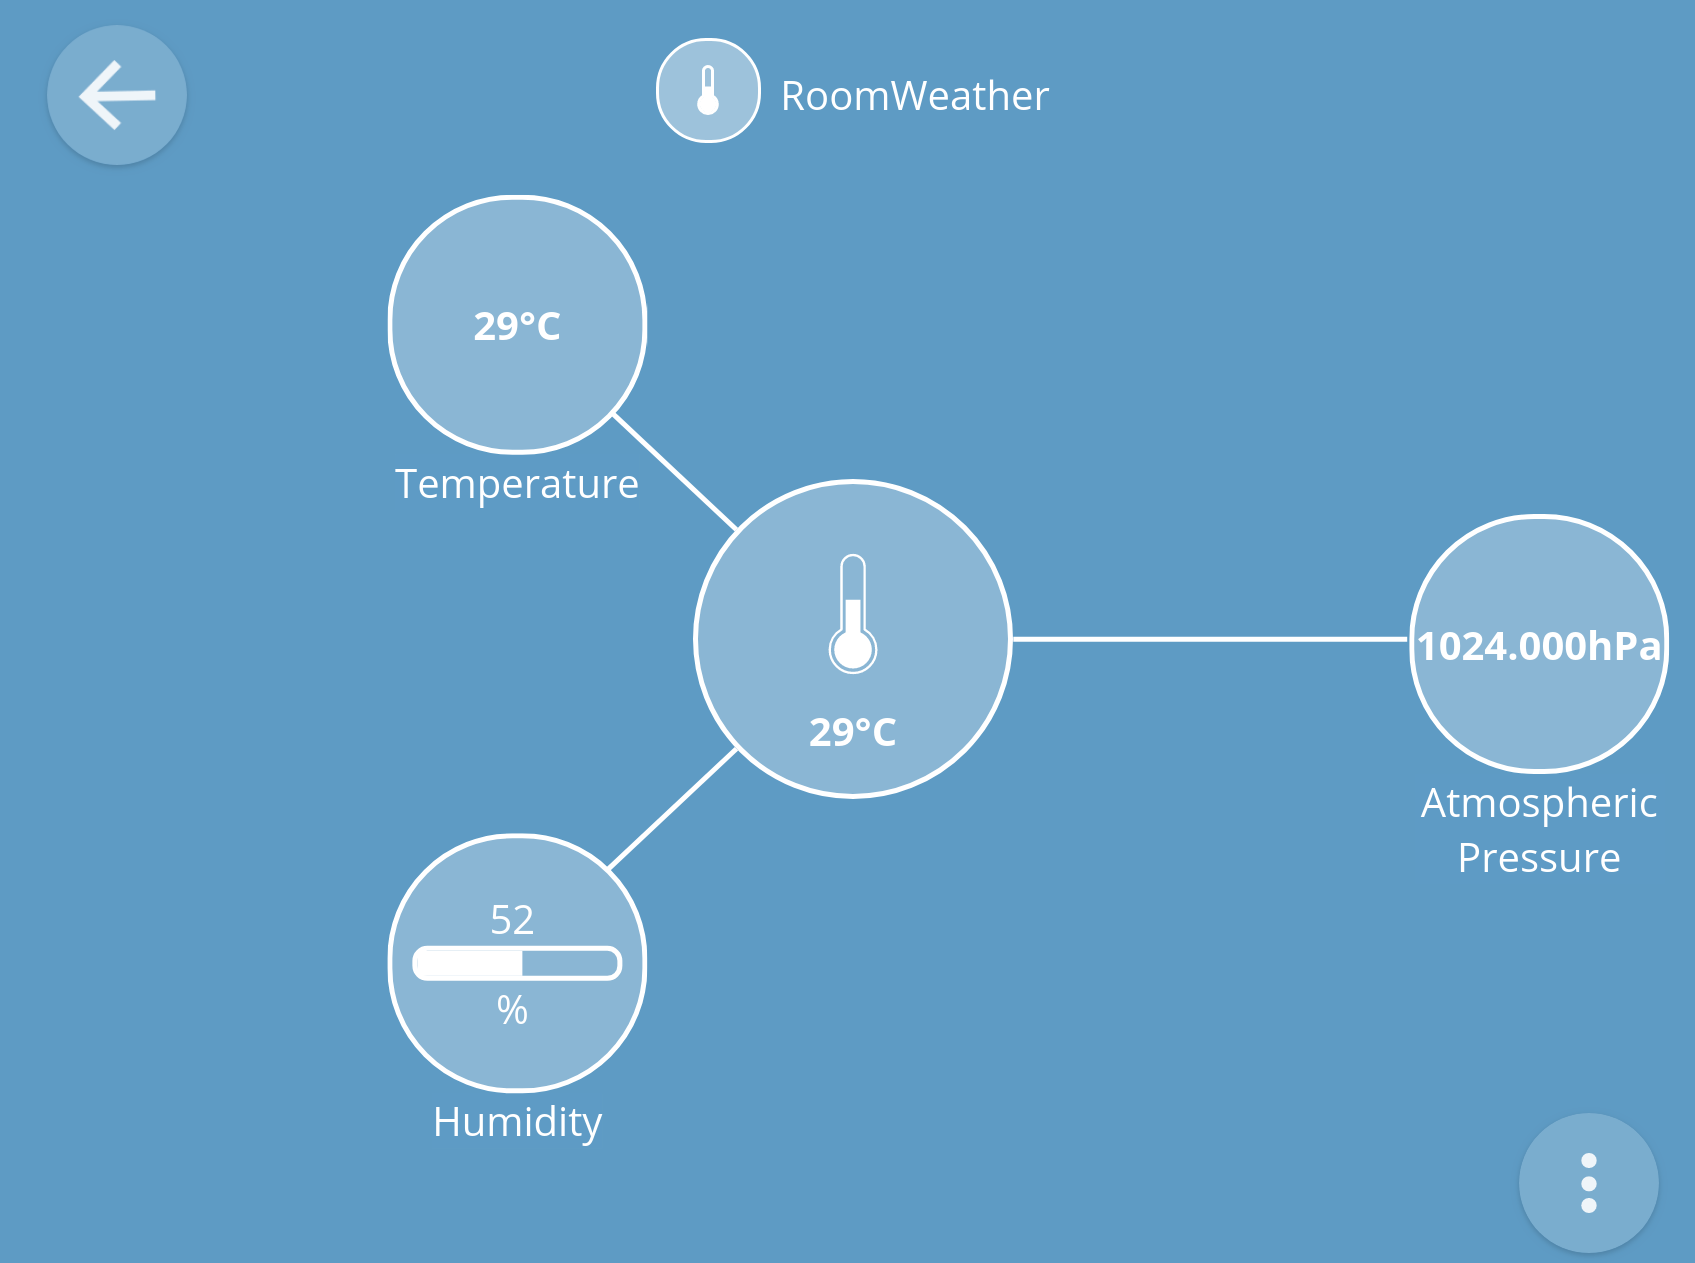
\includegraphics[width=8cm]{img/RoomWeather.png}
    \caption{Visualizzazione di Room Weather come web thing attraverso il Gateway di Mozilla}
    \label{fig:webthingRW}
\end{figure}

\bigskip

\begin{figure}%
    \centering
    \subfloat[Vista chiusa]{{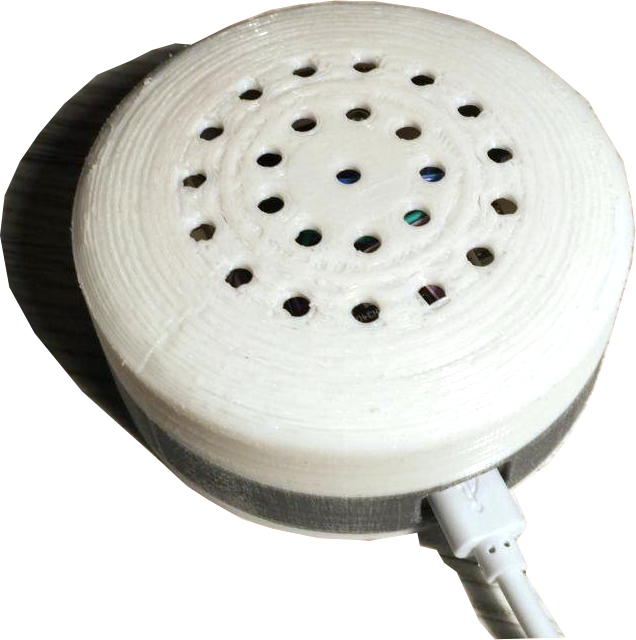
\includegraphics[width=5cm]{img/temp_hum_press_full.png} }}%
    \qquad
    \subfloat[Vista aperta]{{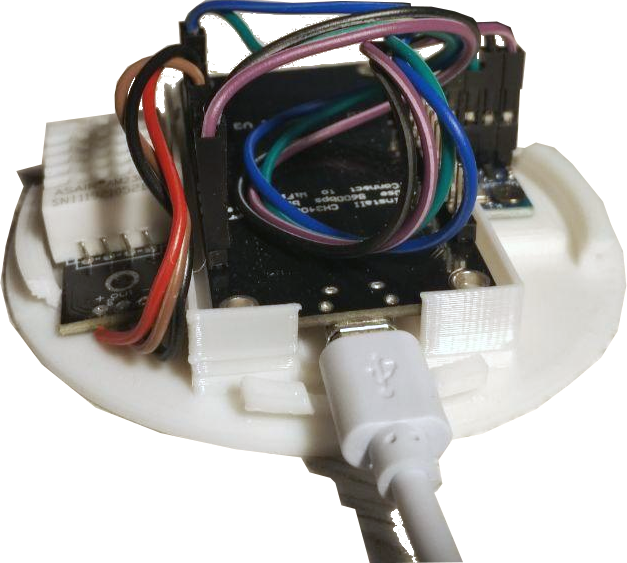
\includegraphics[width=5cm]{img/temp_hum_press_open.png} }}%
    \caption{Viste del sensore Room Weather}
    \label{fig:viewRW}%
\end{figure}

\subsubsection{People Counter}

Per implementare un contatore del numero di persone in prima istanza è stata effettuata una ricerca per valutare le possibili componenti da utilizzare: 

\begin{itemize}
    \item Un sensore Grid-Eye;
    \item Sensori ad infrarossi passivi (PIR);
    \item Sensori anticollisione ad infrarossi; 
    \item Fotoresistenze abbinate a laser.
\end{itemize}

Il sensore Grid-Eye è composto da una griglia di 8x8 sensori termici che permettono di visualizzare una matrice termica dell'area verso cui il sensore è rivolto. Nonostante il potenziale l'ipotesi di utilizzarlo è stata subito scartata per ragioni di costo sia economico che computazionale infatti si sarebbe resa necessaria un'analisi di immagini per poter differenziare eventi di entrata ed uscita.

Assumendo che le entrate/uscite dalla stanza avvengano con il passaggio di una persona alla volta, è possibile passare in analisi anche le altre tipologie di sensori.

Si è passati dunque allo studio dei sensori PIR. Anche quest'ultimi sono stati scartati a causa della scarsa precisione sopratutto quando ravvicinati. 

Sono infine stati realizzati due prototipi utilizzando le ultime due tecnologie passate in rassegna.

Il primo prototipo è stato realizzato utilizzando due sensori anticollisione ad infrarossi (Figura \ref{fig:anticollision}).
Tuttavia questi venivano facilmente influenzati dalla luce solare ed inoltre si sono rivelati essere efficaci solo a brevi distanze (sotto i 20 cm).

\begin{figure}
    \centering
    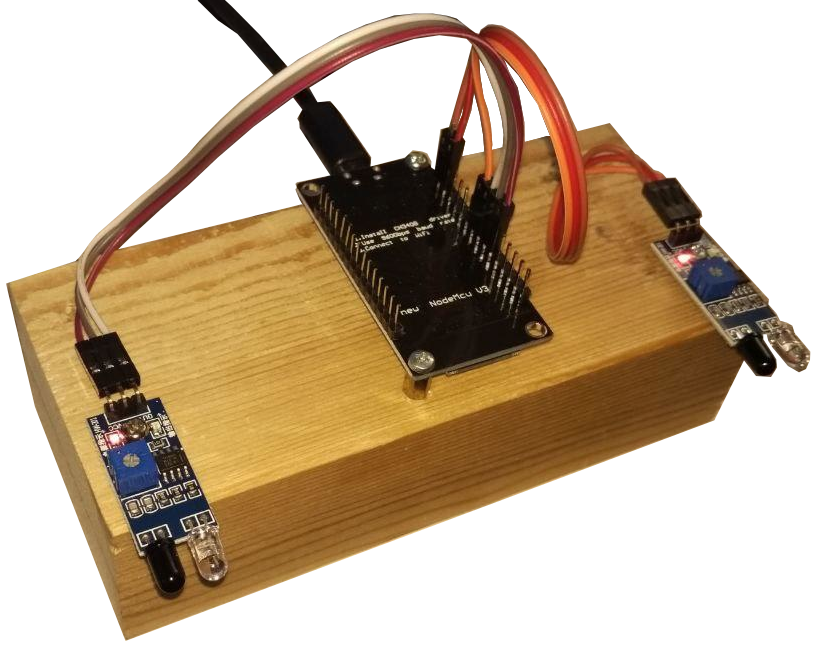
\includegraphics[width=8cm]{img/ir_counter.png}
    \caption{Prototipo per PeopleCounter con sensori anticollisione.}
    \label{fig:anticollision}
\end{figure}

Con poche modifiche è stato realizzato il secondo nonché ultimo prototipo utilizzando:
\begin{itemize}
    \item Due laser
    \item Due fotoresistenze
\end{itemize}

L'idea di base per l'implementazione è quella di puntare i laser contro le fotoresistenze per poi controllare quale fascio venga interrotto per primo. Questo permette di dedurre quando il passaggio attraverso una porta sia un evento di entrata o di uscita.

Come per il caso precedente, People Counter è stato implementato come una Web Thing utilizzando il Framework fornito da Mozilla. In particolare è stato definita una thing \textit{People Counter} con una property \textit{peopleNum} che mantiene il numero di persone all'interno del locale.
Di seguito si mostra la thing description ottenuta:

\bigskip
\begin{lstlisting}[language=json,firstnumber=1]
{
    "title": "People Counter Sensors",
    "@context": "https://iot.mozilla.org/schemas",
    "@type": ["MotionSensor"],
    "description": "Counter for people in a room",
    "href": "/things/http---w25.local-things-peopleCounter",
    "properties": {
        "peopleNum": {
            "title": "PeopleCounter",
            "type": "integer",
            "readOnly": true,
            "links": [{ ... }]
        }
    },
    "actions": {},
    "events": {},
    ...
}
\end{lstlisting}
\bigskip

La gestione degli accessi a livello software è stata gestita attraverso interrupt e un timer. Gli interrupt permettono di notificare quando il fascio laser viene interrotto, si valuta quindi se è già stato generato l'interrupt dell'altro laser per capire se il passaggio sia in entrata o in uscita. Il timer è stato introdotto per gestire il caso in cui venga attraversato un solo laser per poi tornare indietro. Nel momento in cui il primo fascio laser viene interrotto, viene avviato un timer entro il quale attendere un interrupt dalla seconda fotoresistenza e, allo scadere del timer, i valori vengono resettati e quindi si ritorna in uno stato in cui nessun fascio laser è stato interrotto.

In Figura \ref{fig:webthingPC} è possibile vedere la visualizzazione attraverso il Mozilla Gateway della web thing People Counter.

\begin{figure}
    \centering
    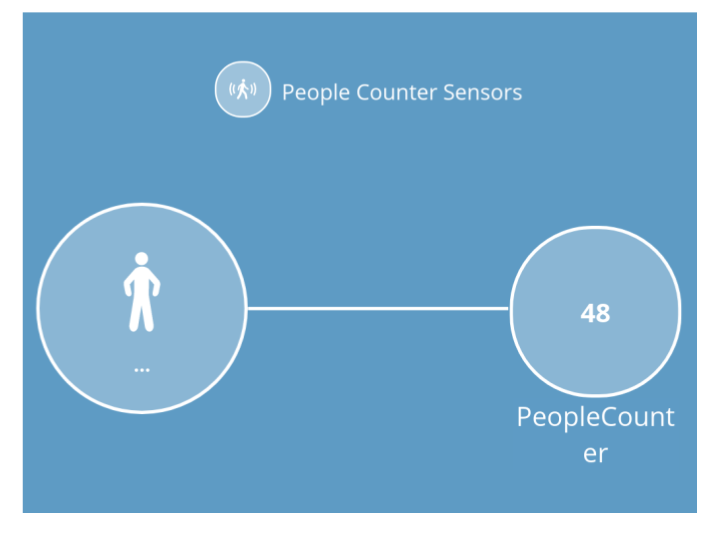
\includegraphics[width=8cm]{img/PeopleCounter.png}
    \caption{Visualizzazione di People Counter come web thing attraverso il Mozilla Gateway}
    \label{fig:webthingPC}
\end{figure}


Anche in questo caso è stato costruito un prototipo di custodia per contenere i laser e le fotoresistenze come è possibile vendere in Figura \ref{fig:viewPC}.

\begin{figure}%
    \centering
    \subfloat[Custodia laser]{{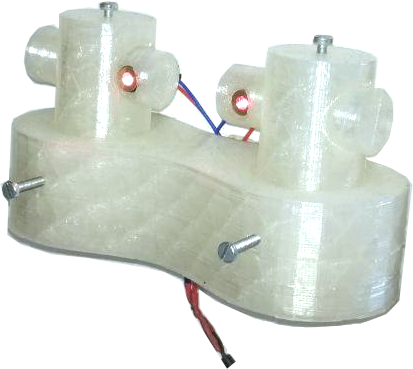
\includegraphics[width=6.5cm]{img/laser.png} }}%
    \qquad
    \subfloat[Custodia receiver]{{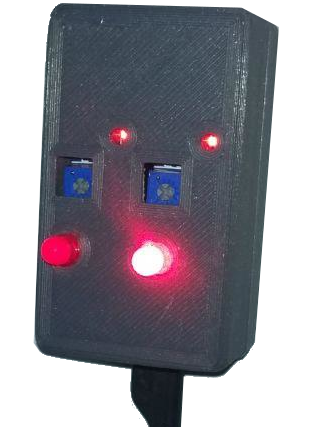
\includegraphics[width=3.5cm]{img/photoresistor.png} }}%
    \caption{Viste della custodia per People Counter}
    \label{fig:viewPC}%
\end{figure}


\subsubsection{WoT Thing aggiuntive}
Inoltre sono state utilizzate altre due thing ottenute attraverso un add-on del Mozilla Gateway che permettono di monitorare le condizioni del Raspberry Pi 3. In particolare una thing permette di monitorare la temperatura della CPU e l'utilizzo della RAM. 
L'utilizzo di queste thing è stato rilevante perché il Raspberry Pi mostrava crash piuttosto frequenti che sono stati ricondotti a un eccessivo surriscaldamento. Per questo motivo è stato ideato un sistema di raffreddamento che ha permesso il proseguimento del lavoro. In Figura \ref{fig:raspberry} si mostra il Raspberry con la ventola dedicata al raffreddamento che ha permesso di abbassare di circa 10 gradi la temperatura del sistema.
\begin{figure}
    \centering
    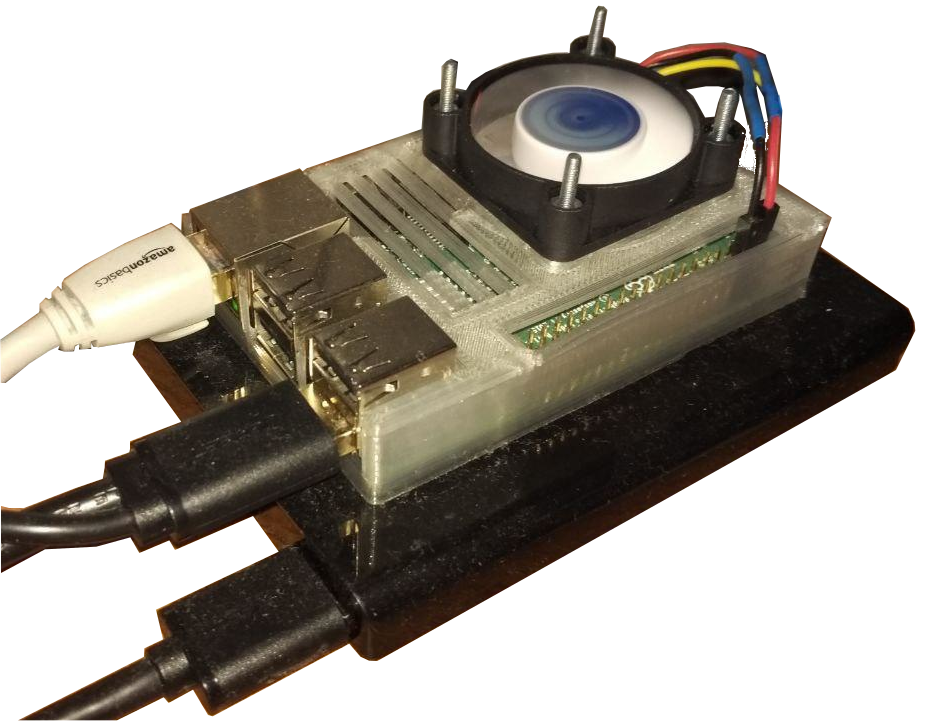
\includegraphics[width=8cm]{img/raspberry.png}
    \caption{Raspberry Pi 3 utilizzato e ventola per il raffreddamento}
    \label{fig:raspberry}
\end{figure}


\subsection{Mozilla Gateway}
Il Mozilla Gateway è stato utilizzato perché risolve il problema della findablity delle things. 

Nel momento in cui si vuole effettuare una ricerca delle thing, il gateway di Mozilla fornisce una funzione di search che utilizza il protocollo mDNS per capire quali siano i device connessi alla rete locale. Trovati tutti i device, è possibile selezionare quello da aggiungere e di questo ne viene effettuata una copia sul gateway stesso.
L'indirizzo IP del device viene però sostituito con quello di ritorno del protocollo mDNS, in questo modo le thing sono esposte all'esterno attraverso il gateway su cui viene anche implementato lo strato di sicurezza. 

Inoltre il Mozilla Gateway è in grado di gestire la riconnessione delle thing.


\subsection{InfluxDB bridge}

Per connettere il Gateway di Mozilla a InfluxDB  è stato scritto un add-on partendo dall'implementazione, disponibile su GitHub, di Tim Hellhake \cite{influxdbBridge} che però è stata modificata per aggiungere compatibilità con InfluxDB 2.0. Sono state inoltre aggiunte alcune funzionalità che non erano presenti nell'add-on originale, in particolare la possibilità di selezionare quali Thing salvare e la possibilità di riconnetersi automaticamente nel caso in cui la thing si sia per qualche motivo disconnessa.


L'add-on è in grado di ottenere dal Mozilla Gateway la lista dei device presenti e di eseguire un'operazione di filtraggio in modo da caricare su InfluxDB le informazioni relative solamente ad alcune thing di interesse.
Per ogni dispositivo viene svolto un tentativo di aprire un websocket e, all'arrivo di messaggi da parte delle thing, viene costruito un nuovo punto da salvare su InfluxDB. 
I punti su InfluxDB sono salvati con il valore, il nome della property e le informazioni relative al device.

In Figura \ref{fig:addon} è possibile visualizzare attraverso il Mozilla Gateway l'add-on costruito. L'add-on necessita di due token, quello per poter leggere dal gateway e quello per poter scrivere su InfluxDB, inoltre gli sono fornite le informazioni principali per poter scrivere sul database di Influx ossia: hostname, port, organization e bucket.

\begin{figure}
    \centering
    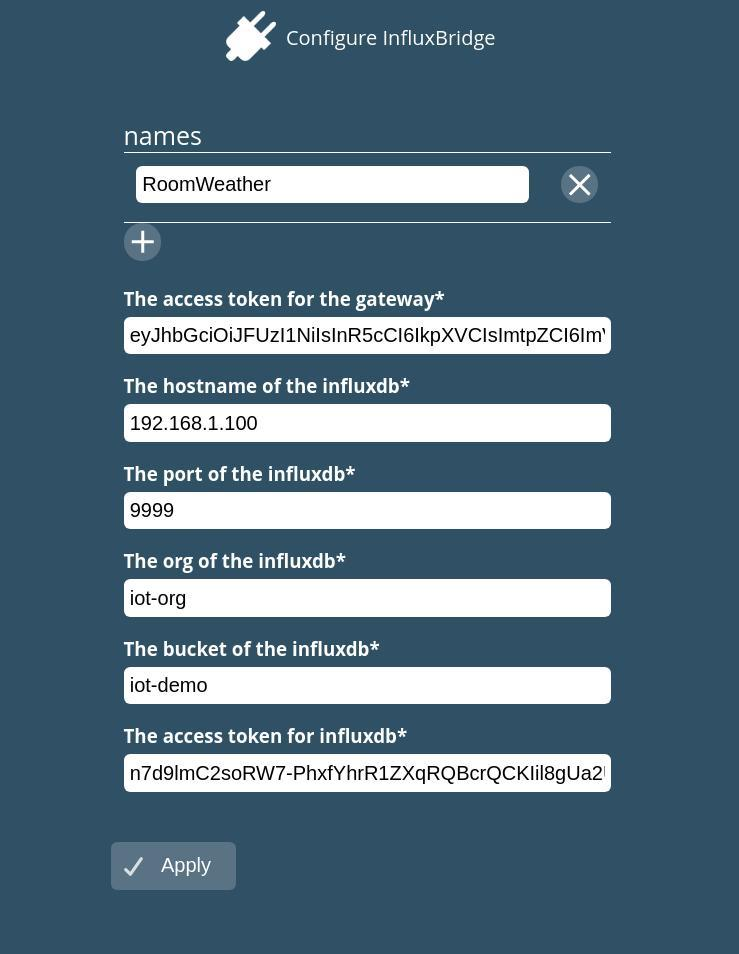
\includegraphics[width=7cm]{img/influx-bridge.jpg}
    \caption{Visualizzazione attraverso il Mozilla Gateway dell'add-on costruito}
    \label{fig:addon}
\end{figure}

\subsection{Analisi dei dati}
Utilizzando Python e Jupyter Notebook è stato possibile interrogare il database di InfluxDB e analizzare il sistema migliore per fare previsioni sui dati. I dati utilizzati consistono di valori raccolti su 12 giorni e aggregati ogni 5 minuti. 

\subsubsection{Pulizia del Dataset}
In una prima fase si utilizza il client di influxDB per richiedere i dati da analizzare ed inserirli in un Dataframe (Figura \ref{fig:df_table}). Utilizzando la libreria di panadas sono state fatte alcune elaborazioni su tale Dataframe per riempire i valori nulli.

\begin{figure}
    \centering
    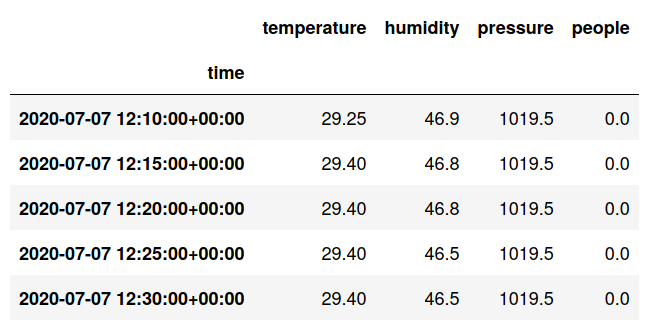
\includegraphics[width=8cm]{img/dfTable.png}
    \caption{Visualizzazione del dataframe ottenuto da InfluxDB}
    \label{fig:df_table}
\end{figure}

\subsubsection{Stazionarietà}
In un secondo momento si è svolta un'analisi per valutare se le serie ottenute fossero o meno stazionarie. Per questo viene utilizzata una funzione che svolga il test Dickey-Fuller. Dai risultati, mostrati in Figura \ref{fig:stazionerietà}, è possibile vedere che la temperatura e il numero di persone sono identificate come serie stazionarie mentre umidità e pressione sono valutate come serie non stazionarie.

\begin{figure}
    \centering
    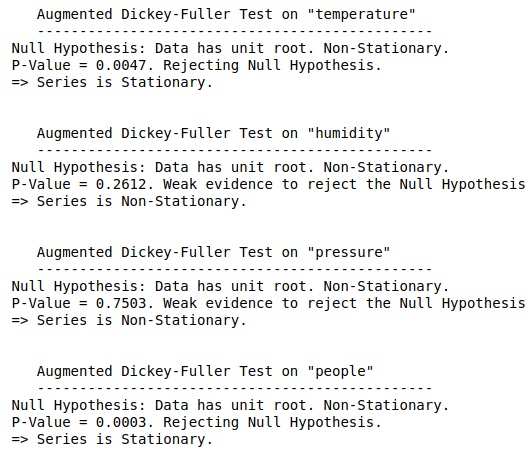
\includegraphics[width=12cm]{img/dickeyFuller.png}
    \caption{Risultati del Dickey-Fuller test su temperatura, umidità, pressione e persone}
    \label{fig:stazionerietà}
\end{figure}

\subsubsection{Componenti della timeseries}
Una serie temporale è costituita da tre componenti:
\begin{enumerate}
    \item Trend: valore crescente o decrescente della serie
    \item Stagionalità: cicli ripetuti nel breve termine all'interno della serie
    \item Rumore: variazione casuale nella serie
\end{enumerate}

Le prime due componenti sono dette sistematiche perché hanno una consistenza o ricorrenza che può essere modellata, l'ultima è detta non sistematica perché la componente del rumore della serie temporale non può essere direttamente modellata. In generale le time-series sono un'aggregazione o combinazione di queste tre componenti.

Le diverse componenti sono state estratte per ognuna delle quattro misurazioni (temperatura, umidità, pressione e numero di persone) e sono rappresentate in Figura \ref{fig:componenti}. In particolare il primo grafico rappresenta il trend della serie, il secondo rappresenta il rumore, il terzo rappresenta la stagionalità e l'ultimo rappresenta la forma effettiva della serie.

\begin{figure}
    \centering
    \subfloat[Analisi delle componenti per i valori di temperatura] {{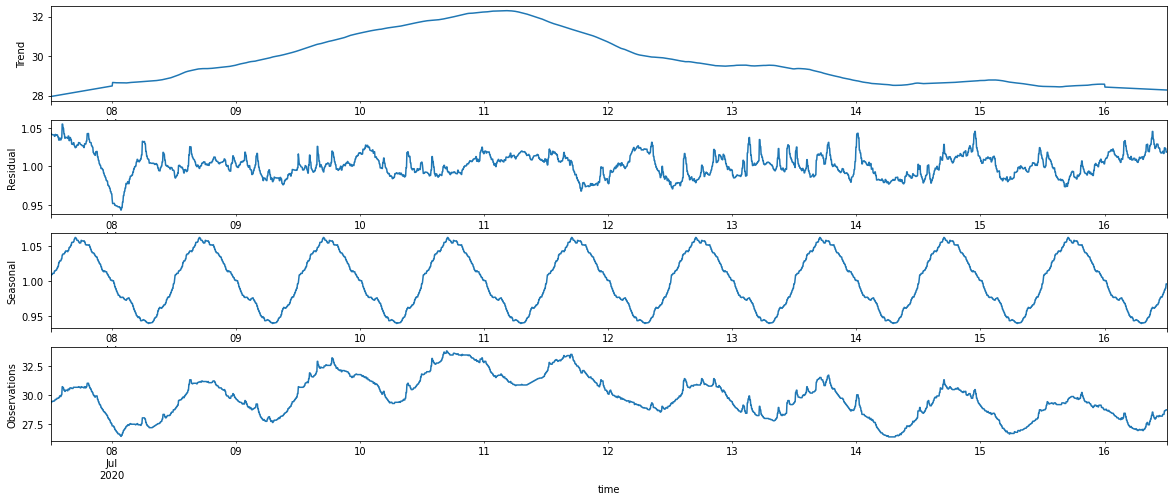
\includegraphics[width=10cm]{img/componentiTemp.png}}}%
    \qquad
    \subfloat[Analisi delle componenti per i valori di umidità]
    {{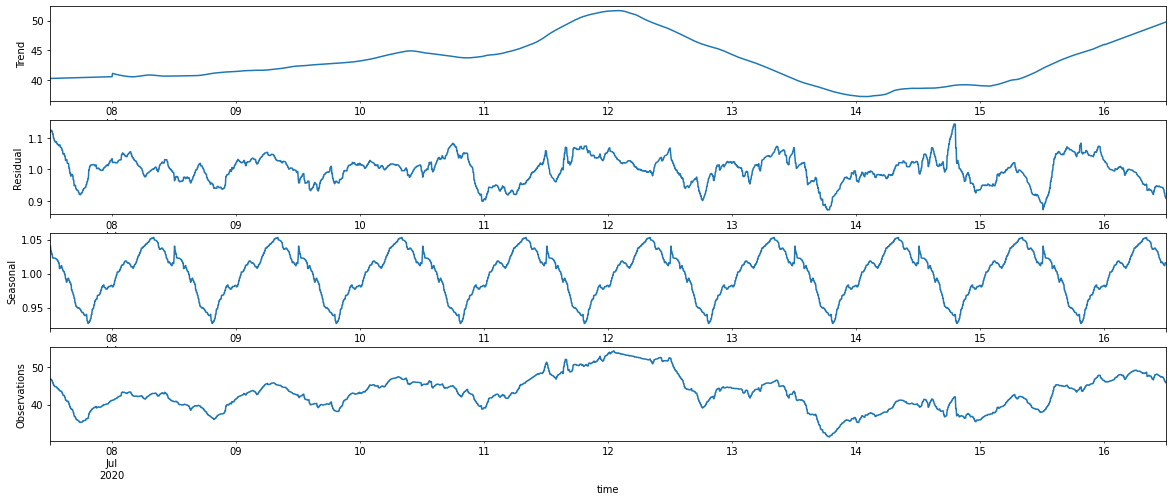
\includegraphics[width=10cm]{img/componentiHum.png}}}%
    \qquad
    \subfloat[Analisi delle componenti per i valori di pressione]
    {{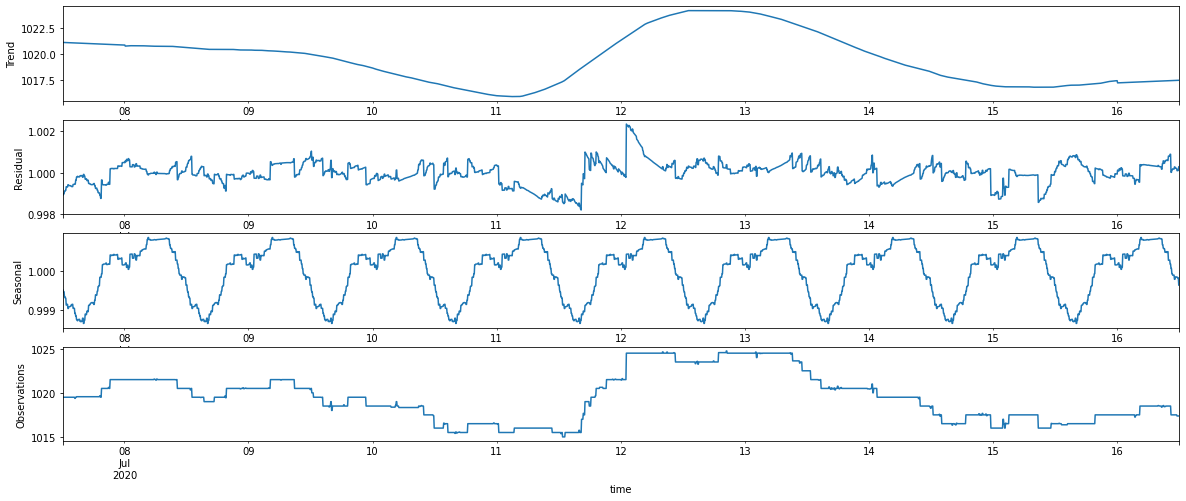
\includegraphics[width=10cm]{img/componentiPress.png}}}%
    \qquad
    \subfloat[Analisi delle componenti per i valori riguardo al numero di persone]
    {{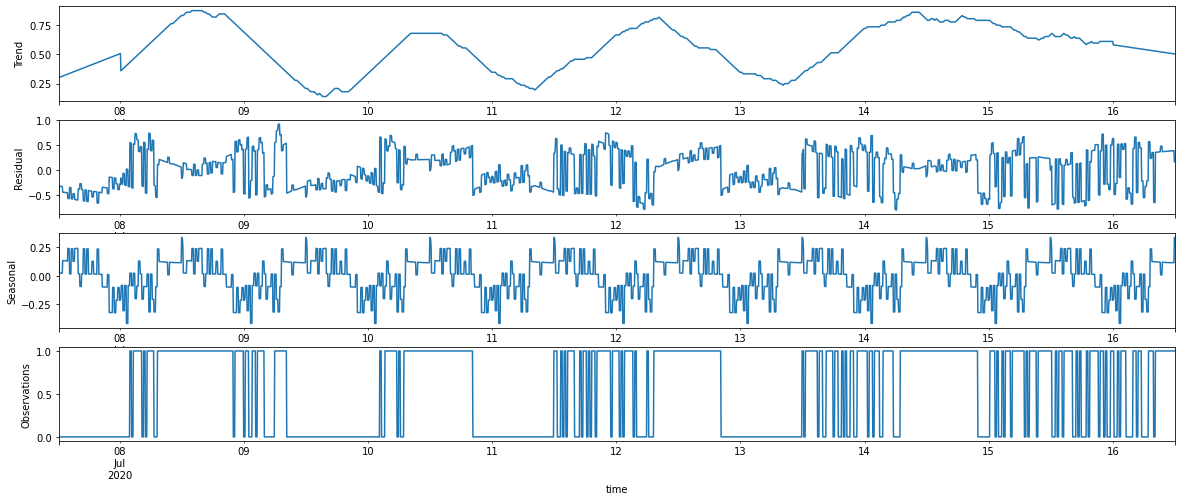
\includegraphics[width=10cm]{img/componentiPeople.png}}}%
    \caption{Analisi delle componenti delle time-series}
    \label{fig:componenti}
\end{figure}



\subsubsection{Autocorrelazione}
La correlazione di Pearson è un coefficiente compreso tra -1 e 1 che descrive una correlazione negativa o positiva rispettivamente. Dato che i fattori ambientali sono influenzati dal momento della giornata, si ipotizza una forte correlazione tra il valore attuale e quello del giorno precedente allo stesso orario. Per valutare ciò sono state utilizzate una funzione di autocorrelazione (ACF) e autocorrelazione parziale (PACF). In Figura \ref{fig:correlazione} sono mostrati i grafici di ACF e PACF per i valori della temperatura.

Il grafico in Figura \ref{fig:correlazioneA} mostra la correlazione della temperatura attuale con i valori precedenti di temperatura. Risulta possibile notare che la temperatura è fortemente correlata ai valori che la precedono e che, allontanandosi nel tempo, la correlazione diminuisce. Inoltre si può osservare come la correlazione, il giorno precedente nella stessa fascia oraria, sia molto elevata.

Per valutare l'effettiva correlazione tra due punti indipendentemente dalla correlazione che deriva dai valori vicini, si utilizza il grafico PACF. Il grafico in Figura \ref{fig:correlazioneB} ci mostra come il valore attuale di temperatura sia fortemente correlato a quello subito precedente e a quello prima. Sul grafico PACF è possibile svolgere un ragionamento analogo anche per i grafici ottenuti dall'analisi di umidità e pressione in cui il valore attuale è fortemente collegato solamente a pochi valori che lo precedono.


\begin{figure}%
    \centering
    \subfloat[Grafico ACF per la temperatura ]{{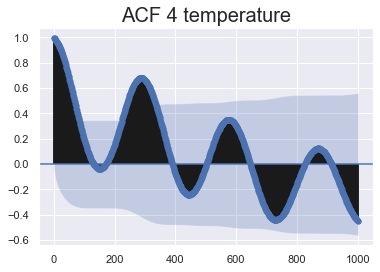
\includegraphics[width=5.5cm]{img/acfTemp.png} \label{fig:correlazioneA}}}%
    \qquad
    \subfloat[Grafico PACF per la temperatura ]{{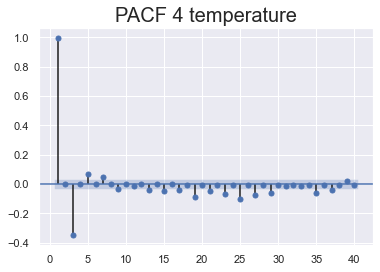
\includegraphics[width=5.5cm]{img/pacfTemp.png} \label{fig:correlazioneB}}}%
    \caption{Grafici di correlazione per i valori di temperatura}
    \label{fig:correlazione}
\end{figure}

\subsection{Metodi di forecasting testati}

Sono stati testati diversi metodi per fare previsione sui dati ottenuti dai sensori. In particolare sono state testate le seguenti metodologie:
\begin{itemize}
    \item Seasonal Autoregressive Integrated Moving-Average (SARIMA)
    \item Vector Autoregression Moving-Average (VARMA)
    \item Holt Winter’s Exponential Smoothing (HWES) 
    \item Long Short-Term Memory (LSTM)
\end{itemize}

\subsubsection{SARIMA}

\textbf{Autoregressive Model (AR)}
\medskip

Il nome del modello AR deriva da autoregressione che significa utilizzare i valori precedenti della variabile per predire i valori futuri. Ci si affida a modelli di autoregressione se esiste una chiara autocorrelazione tra i dati. Il modello può essere rappresentato con parametro 1 dalla formula che segue\cite{arima}:

$$x_t = c + \Phi x_{t-1} + \epsilon_t$$

Dove $x_t$ e $x_{t-1}$ sono rispettivamente il valore attuale e il precedente, $\phi$ è una costante per cui moltiplicare il valore del lag precedente e $\epsilon_t$  è il residuo, ossia la differenza tra la predizione e il valore reale.

Analizzando il grafico PACF per la temperatura (Figura \ref{fig:correlazioneB}) risulta possibile verificare che i valori di correlazione sono significativi fino al terzo valore, graficamente sono riconosciuti come significativi i punti fuori dall'area azzurra. Si ricerca quindi un valore di AR minore o uguale a 3. Per questo motivo sono stati testati AR(1), AR(2) e AR(3). Analizzando i coefficienti ottenuti, è possibile verificare che per tutti i modelli testati, siano tutti sono significativi. Si è utilizzata una funzione ausiliaria per testare se la likelihood del modello più complesso (AR(3)) fosse significativamente migliore rispetto a quella dei modelli più semplici  (AR(1)). Dato che il miglioramento è significativo, si sceglie come migliore il modello AR(3).

In Figura \ref{fig:ar} è possibile vedere i risultati ottenuti utilizzando il modello AR sui valori di temperatura, umidità e pressione. In blu sono mostrati i valori attesi mentre in rosso quelli ottenuti con la previsione del modello AR. In Tabella \ref{tab:ar} è possibile vedere i calcoli dell'errore medio assoluto (MAE) e dell'errore medio quadrato (MSE).

I risultati ottenuti per i valori di temperature (Figura \ref{fig:arTemp}) sono considerati buoni per quanto riguarda il MSE, ma si è voluto cercare un modello più complesso che permettesse di approssimare in maniera più efficace l'andamento dei valori della temperatura.

Per quanto riguarda l'umidità (Figura \ref{fig:arHum}) e la pressione (Figura \ref{fig:arPress}) sono stati svolti ragionamenti analoghi a quelli svolti sulla temperatura per trovare il parametro ottimale per il modello AR, ma per queste misurazioni l'MSE riscontrato è risultato troppo elevato per potersi considerare soddisfatti di un modello così semplice.

\begin{table}
\centering
\arrayrulecolor{black}
\begin{tabular}{l|r|r|r|r}
\multicolumn{5}{c}{{\cellcolor[rgb]{0.875,0.875,0.875}} Metodo AR}\\ 
\hline
\rowcolor[rgb]{0.753,0.753,0.753}             
& \multicolumn{2}{c|}{\textbf{ 2 h}}              
& \multicolumn{2}{c}{\textbf{24 h }}\\ 
\rowcolor[rgb]{0.753,0.753,0.753}             & \multicolumn{1}{l}{\textbf{MAE}} & \textbf{MSE} & \multicolumn{1}{l|}{\textbf{MAE}} & \multicolumn{1}{c}{\textbf{MSE}}  \\ 
\hline
\rowcolor[rgb]{0.875,0.875,0.875} temperatura & 0.156                            & 0.038        & 0.550                             & 0.392                             \\
umidità                                       & 0.684                            & 0.607        & 2.192                             & 8.942                             \\
\rowcolor[rgb]{0.875,0.875,0.875} pressione   & 0.067                            & 0.005        & 2.075                             & 5.859                            
\end{tabular}
\caption{MAE e MSE ottenuto dalle predizioni di 2 ore e 24 ore sui dati di temperatura, umidità e pressione utilizzando il metodo AR e un training set di 12 giorni}
\label{tab:ar}
\end{table}


\begin{figure}
    \centering
    \subfloat[Predizioni AR per 24 ore sui valori di temperature] {{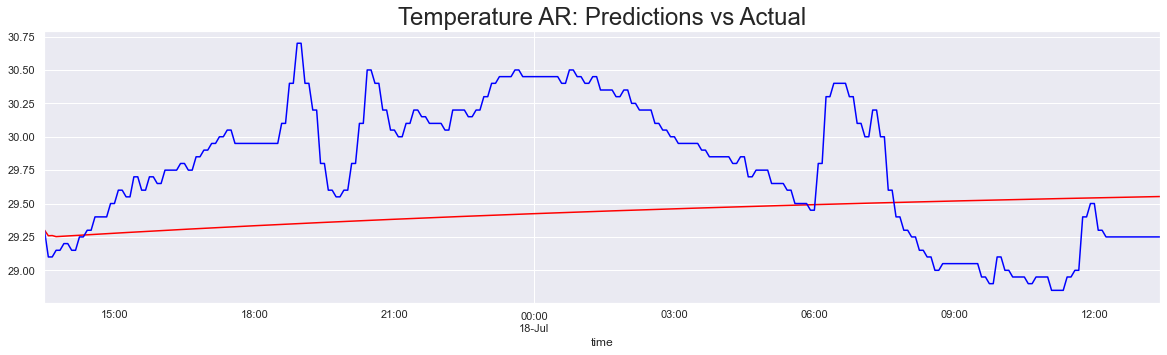
\includegraphics[width=12cm]{img/arTemp.png} \label{fig:arTemp}}}%
    \qquad
    \subfloat[Predizioni AR per 24 ore sui valori di umidità]
    {{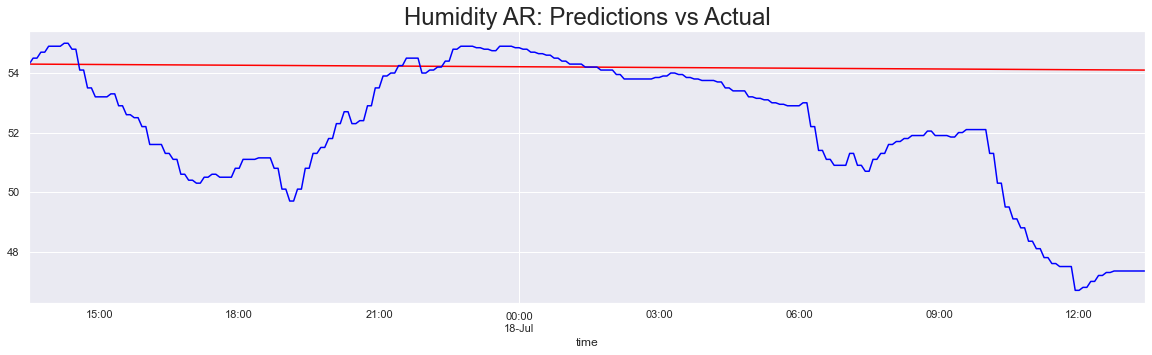
\includegraphics[width=12cm]{img/arHum.png} \label{fig:arHum}}}%
    \qquad
    \subfloat[Predizioni AR per 24 ore sui valori di pressione]
    {{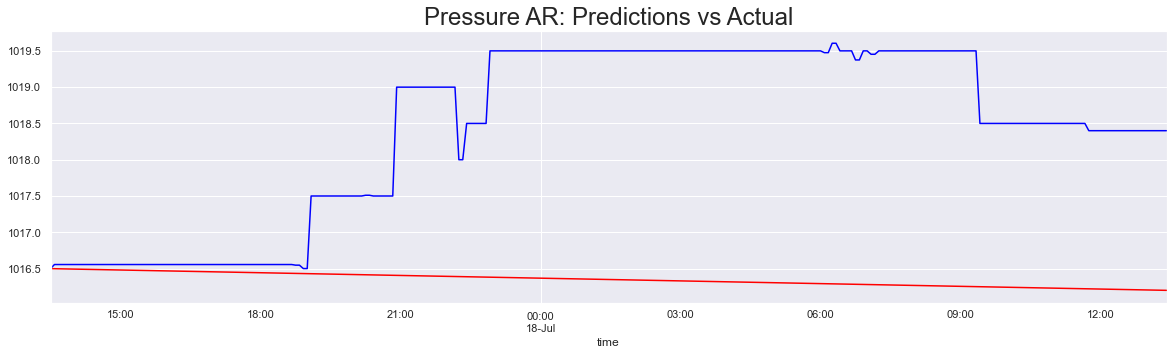
\includegraphics[width=12cm]{img/arPress.png}
    \label{fig:arPress}}}%
    \caption{Previsioni ottenute dal modello AR applicato ai dati di 11 giorni di temperatura, umidità e pressione per l'arco di una giornata. In rosso sono mostrati i valori predetti e in blu quelli attesi.}
    \label{fig:ar}
\end{figure}


\bigskip
\textbf{Moving Average Model (MA)}
\medskip

Il modello viene utilizzato nel caso in cui ci siano altri fattori oltre ai valori precedenti delle variabili che devono essere tenuti in considerazione. Pertanto, sapendo l'errore nelle previsioni precedenti, è possibile stimare in maniera migliore i nuovi valori. Questo è il motivo per cui i modelli MA incorporano i residui dei valori passati per migliorare le stime future. I modelli MA permettono di gestire in maniera più efficace gli imprevisti, per questo motivo sono noti come modelli di smoothing. Un MA di parametro 1 è definito attraverso la seguente formula\cite{arima}:
$$r_t = c + \Theta_1\epsilon_{t-1} + \epsilon_t$$
Dove $r$ è il valore attuale stimato, $\Theta_1$ è il coefficiente associato al primo lag, $\epsilon_t$ e $\epsilon_{t-1}$ sono rispettivamente il valore residuo per il periodo corrente e il periodo precedente.

\begin{table}
\centering
\begin{tabular}{l|r|r|r|r}
\multicolumn{5}{c}{{\cellcolor[rgb]{0.875,0.875,0.875}} Metodo MA}                                                                                                                            \\ 
\hline
\rowcolor[rgb]{0.753,0.753,0.753}             & \multicolumn{2}{c|}{\textbf{ 2 h}}                                    & \multicolumn{2}{c}{\textbf{24 h }}                                    \\
\rowcolor[rgb]{0.753,0.753,0.753}             & \multicolumn{1}{c|}{\textbf{MAE}} & \multicolumn{1}{c|}{\textbf{MSE}} & \multicolumn{1}{c|}{\textbf{MAE}} & \multicolumn{1}{c}{\textbf{MSE}}  \\ 
\hline
\rowcolor[rgb]{0.875,0.875,0.875} temperatura & 0.350                             & 0.156                             & 0.426                             & 0.242                             \\
umidità                                       & 9.886                             & 100.737                           & 2.192                             & 74.885                            \\
\rowcolor[rgb]{0.875,0.875,0.875} pressione   & 2.262                             & 5.592                             & 2.075                             & 1.825                            
\end{tabular}
\caption{MAE e MSE ottenuto dalle predizioni di 2 ore e 24 ore sui dati di temperatura, umidità e pressione utilizzando il metodo MA e un training set di 12 giorni}
\label{tab:ma}
\end{table}


In Figura \ref{fig:ma} è possibile vedere i risultati ottenuti applicando MA ai dati di temperatura, umidità e pressione, in blu sono mostrati i valori attesi mentre in rosso i valori predetti dal modello. In Tabella \ref{tab:ma} sono mostrati gli errori MAE e MSE. Il MSE ottenuto è buono per i valori di temperatura, ma non per quelli di umidità e pressione. Inoltre in tutti i casi la previsione consiste fondamentalmente di una linea retta e non è in grado di seguire l'andamento dei dati.

Per questo motivo sono stati tentati approcci più complessi.



\begin{figure}
    \centering
    \subfloat[Predizioni MA per 24 ore sui valori di temperature] {{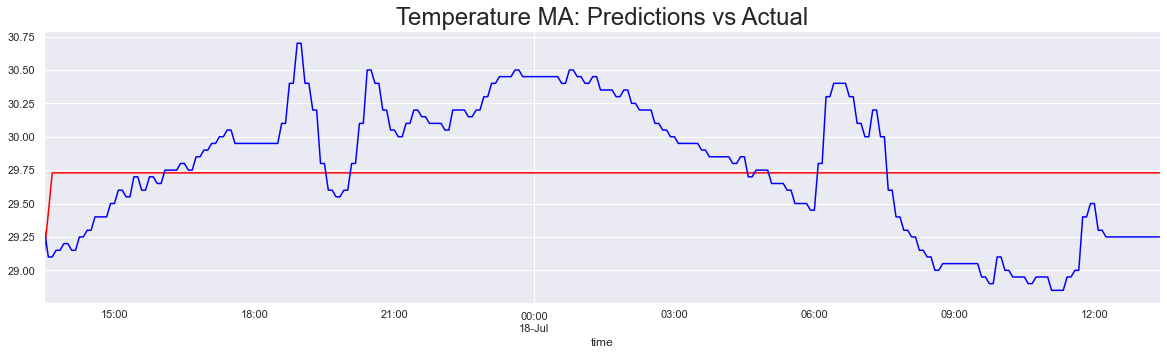
\includegraphics[width=12cm]{img/maTemp.png} \label{fig:maTemp}}}%
    \qquad
    \subfloat[Predizioni MA per 24 ore sui valori di umidità]
    {{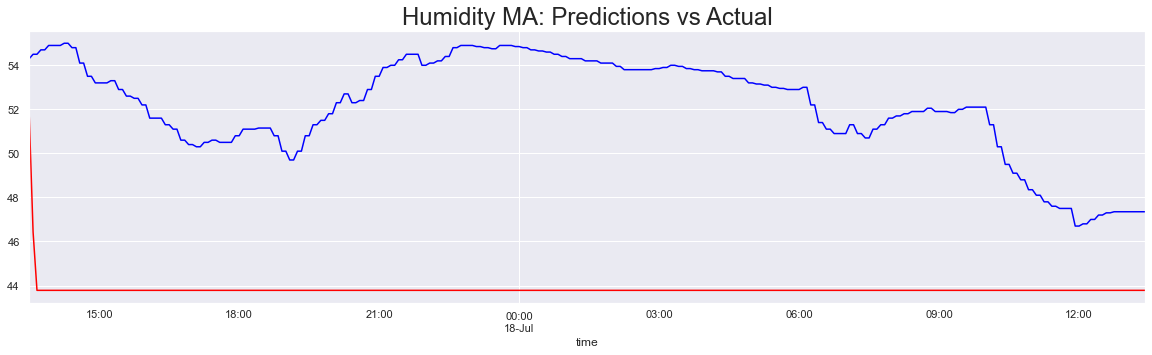
\includegraphics[width=12cm]{img/maHum.png} \label{fig:maHum}}}%
    \qquad
    \subfloat[Predizioni MA per 24 ore sui valori di pressione]
    {{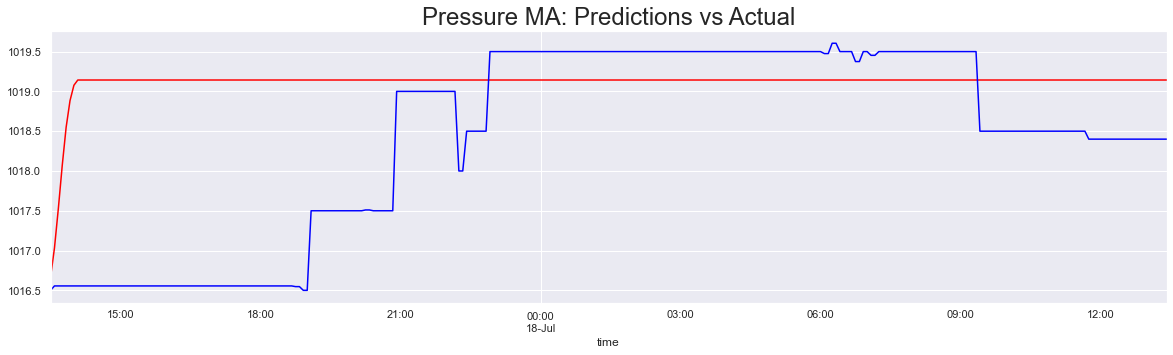
\includegraphics[width=12cm]{img/maPress.png}
    \label{fig:maPress}}}%
    \caption{Previsioni ottenute dal modello
    MA applicato ai dati di 11 giorni di temperatura, umidità e pressione per l'arco di una giornata. In rosso sono mostrati i valori predetti e in blu quelli attesi.}
    \label{fig:ma}
\end{figure}


\bigskip
\textbf{ARMA}
\medskip

Si è passati all'analisi del modello ARMA che permette di combinare i benefici di AR e MA. AR infatti permette di effettuare buone previsioni sui dati stazionari, ma è fallimentare nella gestione degli imprevisti, MA permette di mitigare questo side-effect. Il modello ARMA con parametri (1,1) è rappresentato dalla seguente equazione\cite{arima}:
$$r_t = c + \Phi r_{t-1} + \Theta_1\epsilon_{t-1} + \epsilon_t$$

Dove $r_t$ e $r_{t-1}$ sono i valori attuale e precedente, $\epsilon_t$ e $\epsilon_{t-1}$ sono rispettivamente il valore residuo per il periodo corrente e il periodo precedente, $\Theta_1$ e $\Phi$ sono due coefficienti che rappresentano rispettivamente quanta parte dell'errore e del valore precedente sono rilevanti nel calcolo del valore successivo.

Seguendo la linea utilizzata negli esperimenti precedenti, si è testato il modello ARMA(p,q) scegliendo $p$ e $q$ in base ai risultati ottenuti nell'elaborazione dei modelli AR e MA. Sono stati quindi selezionati i modelli ARMA(p,q) tali per cui tutti i parametri ottenuti dal modello fossero significativi e quindi non ci fosse rischio di overfitting. Infine è stata analizzata la log likelihood e l'information criteria (AIC) dei modelli rimasti e si è testato il modello che presentasse migliore likelihood e, contemporaneamente, AIC più bassa.

Per i valori di temperatura, umidità e pressione sono stati selezionati rispettivamente i modelli ARMA(2,1), ARMA(2,3) e ARMA(2,1). In Figura \ref{fig:arma} si mostrano i risultati ottenuti dove in rosso sono mostrati i valori predetti e in blu i valori attesi mentre in Tabella \ref{tab:arma} si mostrano i valori di MAE e MSE calcolati.

Per quanto riguarda la temperatura il MSE risulta sempre poco significativo mentre per le altre raccolte di dati è molto elevato. Questo può essere dovuto al fatto che la temperatura è una serie stazionaria mentre l'umidità e la pressione non sono stazionarie. Per questo motivo viene testato il modello ARIMA che dovrebbe essere più efficace nel caso di serie non stazionarie.

\begin{table}
\centering
\begin{tabular}{l|r|r|r|r}
\multicolumn{5}{c}{{\cellcolor[rgb]{0.875,0.875,0.875}} Metodo ARMA}                                                                                                                          \\ 
\hline
\rowcolor[rgb]{0.753,0.753,0.753}             & \multicolumn{2}{c|}{\textbf{ 2 h}}                                    & \multicolumn{2}{c}{\textbf{24 h }}                                    \\
\rowcolor[rgb]{0.753,0.753,0.753}             & \multicolumn{1}{c|}{\textbf{MAE}} & \multicolumn{1}{c|}{\textbf{MSE}} & \multicolumn{1}{c|}{\textbf{MAE}} & \multicolumn{1}{c}{\textbf{MSE}}  \\ 
\hline
\rowcolor[rgb]{0.875,0.875,0.875} temperatura & 0.129                             & 0.022                             & 0.301                             & 0.155                             \\
umidità                                       & 0.495                             & 0.410                             & 2.837                             & 11.465                            \\
\rowcolor[rgb]{0.875,0.875,0.875} pressione   & 0.024                             & 0.001                             & 1.160                             & 2.062                            
\end{tabular}
\caption{MAE e MSE ottenuto dalle predizioni di 2 ore e 24 ore sui dati di temperatura, umidità e pressione utilizzando il metodo ARMA e un training set di 12 giorni}
\label{tab:arma}
\end{table}

 
\begin{figure}
    \centering
    \subfloat[Predizioni ARMA per 24 ore sui valori di temperature]
    {{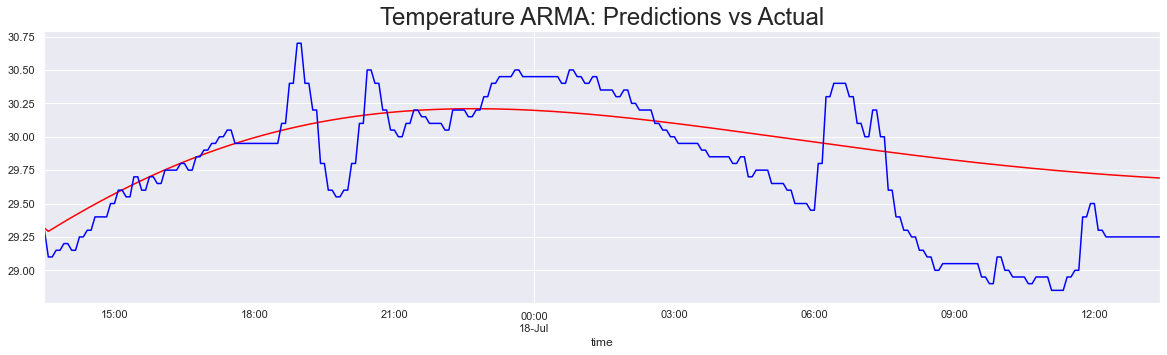
\includegraphics[width=12cm]{img/armaTemp.png} \label{fig:armaTemp}}}%
    \qquad
    \subfloat[Predizioni ARMA per 24 ore sui valori di umidità]
    {{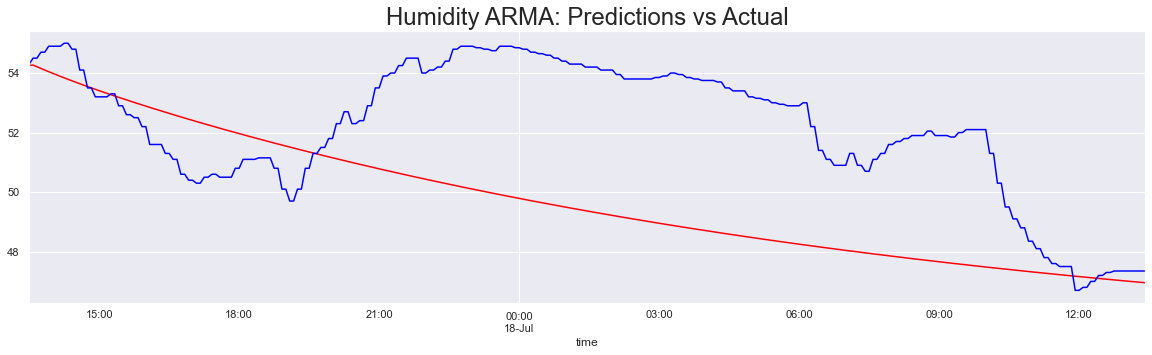
\includegraphics[width=12cm]{img/armaHum.png} \label{fig:armaHum}}}%
    \qquad
    \subfloat[Predizioni ARMA per 24 ore sui valori di pressione]
    {{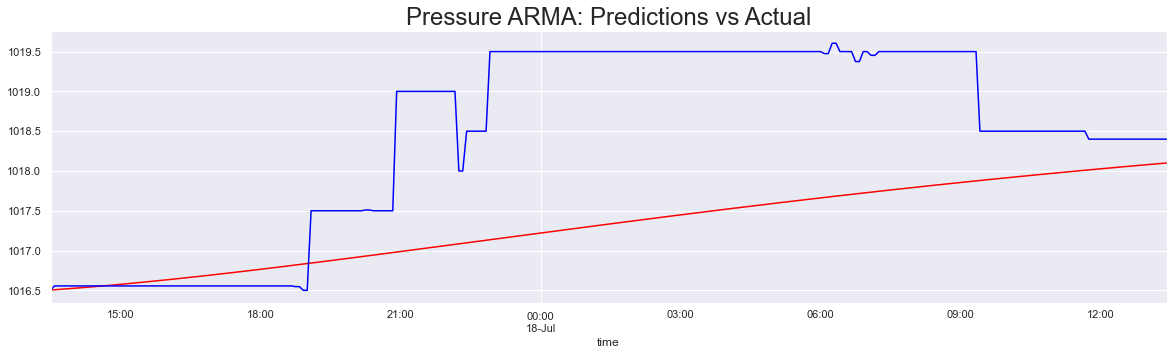
\includegraphics[width=12cm]{img/armaPress.png}
    \label{fig:armaPress}}}%
    \caption{Previsioni ottenute dal modello ARMA applicato ai dati di 11 giorni di temperatura, umidità e pressione per la previsione
    di una giornata. In rosso sono mostrati i valori predetti e in blu quelli attesi.}
    \label{fig:arma}
\end{figure}

\bigskip
\textbf{ARIMA}
\medskip

ARIMA(p,d,q) è una versione integrata del modello ARMA(p,q). Ciò significa che i dati vengono integrati d volte per raggiungere una serie stazionaria.
Il modello ARIMA con parametri (1,1,1) può essere rappresentato dall'equazione che segue\cite{arima}:
$$\Delta P_t = c + \Phi \Delta P_{t-1} + \Theta_1\epsilon_{t-1} + \epsilon_t$$

Dove $\Delta P_t = P_t - P_{t-1}$ e $P_t$ è il valore al tempo $t$, $\epsilon_t$ e $\epsilon_{t-1}$ sono rispettivamente il valore residuo per il periodo corrente e il periodo precedente, $\Theta_1$ e $\Phi$ sono due coefficienti che rappresentano rispettivamente quanta parte dell'errore e del valore precedente sono rilevanti nel calcolo del valore successivo e $c$ è una costante.

Come nei modelli precedenti sono stati testati diversi parametri per ARIMA(p,d,q), sono stati selezionati i modelli che presentavano tutti i coefficienti significativi e tra questi modelli è stato scelto quello con likelihood più alta e AIC  più bassa. Per la temperatura, umidità e pressione sono stati scelti rispettivamente i modelli ARIMA(2,1,1), ARIMA(2,1,3) e ARIMA(2,1,1).

Per quanto riguarda la temperatura, dato che la serie è già risultata stazionaria, l'utilizzo di ARIMA non ha portato a miglioramenti nella likelihood rispetto a modelli più semplici. Anche per i modelli di umidità e pressione però non sono stati riscontrati i miglioramenti attesi. In Tabella \ref{tab:arima} sono mostrati i valori di MAE e MSE ottenuti e in Figura \ref{fig:arima} sono presentati i grafici ottenuti mettendo a confronto i valori attesi (in blu) e quelli predetti (in rosso).

\begin{table}
\centering
\begin{tabular}{l|r|r|r|r}
\multicolumn{5}{c}{{\cellcolor[rgb]{0.875,0.875,0.875}} Metodo ARIMA}                                                                                                                         \\ 
\hline
\rowcolor[rgb]{0.753,0.753,0.753}             & \multicolumn{2}{c|}{\textbf{ 2 h}}                                    & \multicolumn{2}{c}{\textbf{24 h }}                                    \\
\rowcolor[rgb]{0.753,0.753,0.753}             & \multicolumn{1}{c|}{\textbf{MAE}} & \multicolumn{1}{c|}{\textbf{MSE}} & \multicolumn{1}{c|}{\textbf{MAE}} & \multicolumn{1}{c}{\textbf{MSE}}  \\ 
\hline
\rowcolor[rgb]{0.875,0.875,0.875} temperatura & 0.171                             & 0.047                             & 0.603                             & 0.516                             \\
umidità                                       & 0.694                             & 0.667                             & 2.340                             & 9.883                             \\
\rowcolor[rgb]{0.875,0.875,0.875} pressione   & 0.053                             & 0.003                             & 1.924                             & 5.109                            
\end{tabular}
\caption{MAE e MSE ottenuto dalle predizioni di 2 ore e 24 ore sui dati di temperatura, umidità e pressione utilizzando il metodo ARIMA e un training set di 10 giorni}
\label{tab:arima}
\end{table}

\begin{figure}
    \centering
    \subfloat[Predizioni ARIMA per 24 ore sui valori di temperature]
    {{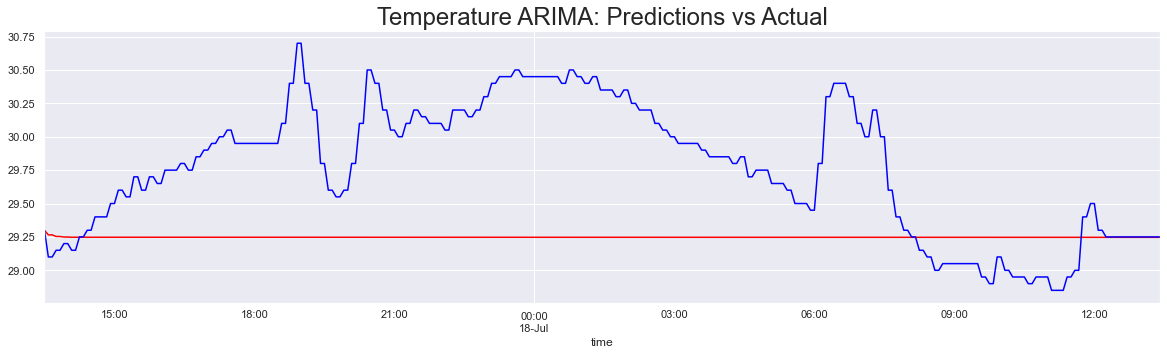
\includegraphics[width=12cm]{img/arimaTemp.png} \label{fig:arimaTemp}}}%
    \qquad
    \subfloat[Predizioni ARIMA per 24 ore sui valori di umidità]
    {{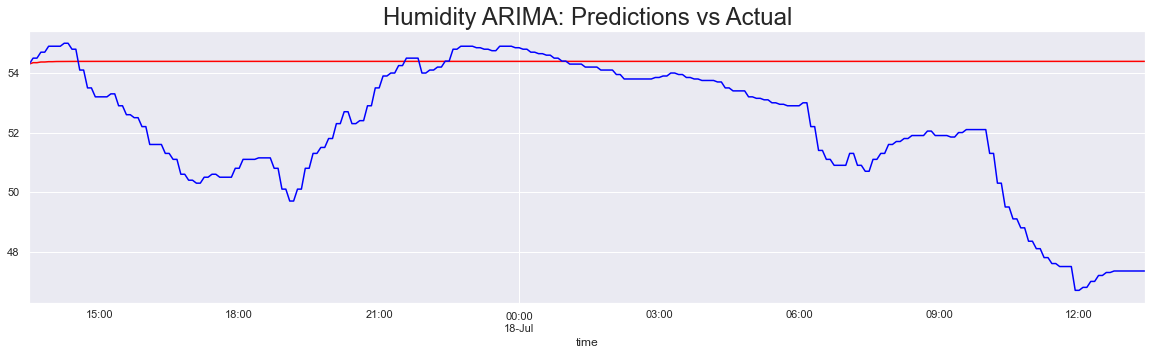
\includegraphics[width=12cm]{img/arimaHum.png} \label{fig:arimaHum}}}%
    \qquad
    \subfloat[Predizioni ARIMA per 24 ore sui valori di pressione]
    {{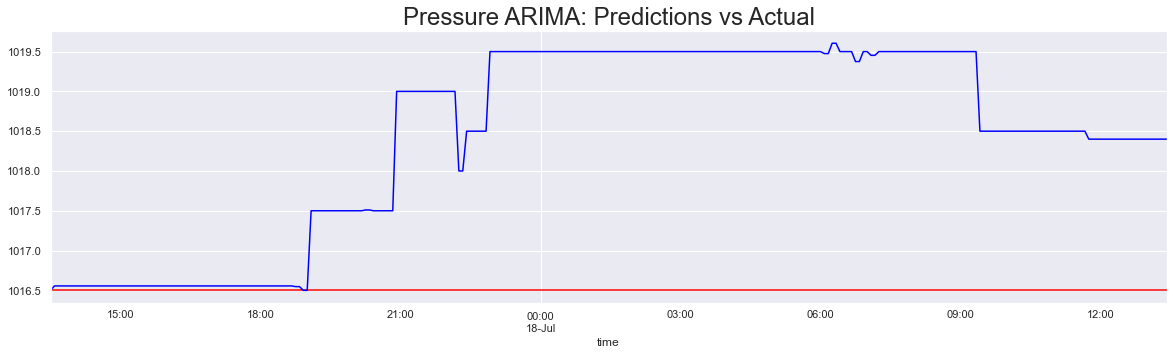
\includegraphics[width=12cm]{img/arimaPress.png}
    \label{fig:arimaPress}}}%
    \caption{Previsioni ottenute dal modello ARIMA applicato ai dati di 11 giorni di temperatura, umidità e pressione per la previsione
    di una giornata. In rosso sono mostrati i valori predetti e in blu quelli attesi.}
    \label{fig:arima}
\end{figure}

\bigskip
\textbf{SARIMA}
\medskip

SARIMA è l'equivalente del modello ARIMA cui viene aggiunta una componente stagionale che permette di catturare pattern che non sono sempre presenti, ma occorrono periodicamente.

Sono stati svolti diversi tentativi di utilizzo del modello SARIMA, ma tale modello, anche con parametri bassi, risulta troppo complesso da calcolare rispetto ai corrispettivi modelli che non presentano stagionalità per questo motivo sono state tentate metodologie diverse. 


\subsubsection{VARMA}
Il metodo Vector Autoregression Moving-Average (VARMA) permette di generalizzare il modello ARMA su più serie temporali in maniera parallela (es. serie temporali multivariate) \cite{varma}. I parametri del modello sono analoghi a quelli utilizzati per AR(p) e MA(q). 

Nel nostro caso specifico è stata utilizzata una versione semplice di VARMA settando il parametro AR e quello MA a 1.

Dato che il modello non presenta una componente di integrazione è stato necessario indurre a mano la stazionarietà delle serie integrando tutte le componenti una volta. 

Il modello sembra adeguato all'utilizzo nel nostro specifico caso d'uso, ma i risultati (Tabella \ref{tab:var}) ottenuti presentano nel caso dell'umidità un MSE molto elevato. In Figura \ref{fig:varma} si mostrano i grafici che mettono a confronto i valori attesi (in blu) con i valori predetti (in rosso) di temperatura, umidità, pressione e numero di persone. Dato che i valori predetti non sono in grado di fornire un'approssimazione dell'andamento dei modelli, si sono tentati approcci diversi.


\begin{table}
\centering
\begin{tabular}{l|r|r|r|r}
\multicolumn{5}{c}{{\cellcolor[rgb]{0.875,0.875,0.875}} Metodo VARMA}                                                                                                                        \\ 
\hline
\rowcolor[rgb]{0.753,0.753,0.753}            & \multicolumn{2}{c|}{\textbf{ 2 h}}                                    & \multicolumn{2}{c}{\textbf{24 h }}                                    \\
\rowcolor[rgb]{0.753,0.753,0.753}            & \multicolumn{1}{c|}{\textbf{MAE}} & \multicolumn{1}{c|}{\textbf{MSE}} & \multicolumn{1}{c|}{\textbf{MAE}} & \multicolumn{1}{c}{\textbf{MSE}}  \\ 
\hline
temperature                                  & 0.186        & 0.040        &0.933        & 1.596         \\
\rowcolor[rgb]{0.875,0.875,0.875} umidità    & 1.981                             & 4.506                             & 2.308                             & 8.391                             \\
pressione                                    & 0.880                             & 0.831                             & 0.731                             & 0.892                             \\
\rowcolor[rgb]{0.875,0.875,0.875} n. persone & 0.625                             & 0.625                             & 0.554                             & 0.554                            
\end{tabular}
\caption{MAE e MSE ottenuti dalle predizioni di 2 ore e di 24 ore sui dati di temperatura, umidità, pressione e numero di persone utilizzando il metodo VARMA e un training set di 12 giorni}
\label{tab:var}
\end{table}


\begin{figure}
    \centering
    \subfloat[Predizioni VARMA per 24 ore sui valori di temperature]
    {{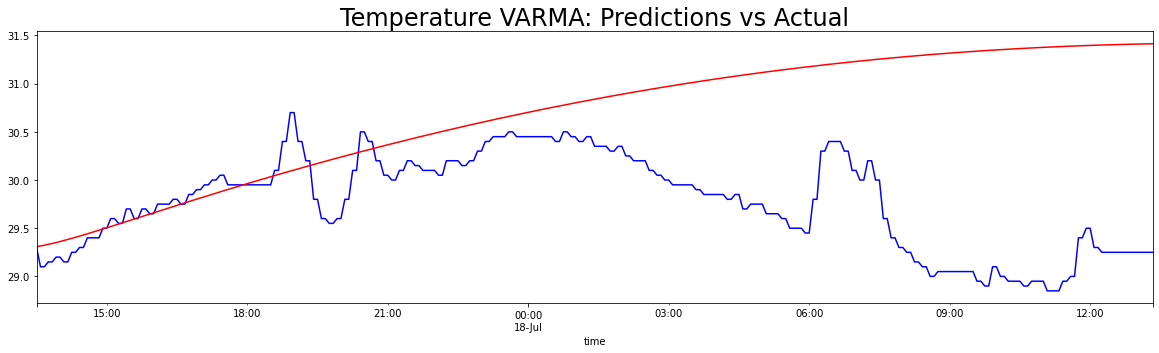
\includegraphics[width=12cm]{img/varmaTemp.png} \label{fig:varmaTemp}}}%
    \qquad
    \subfloat[Predizioni VARMA per 24 ore sui valori di umidità]
    {{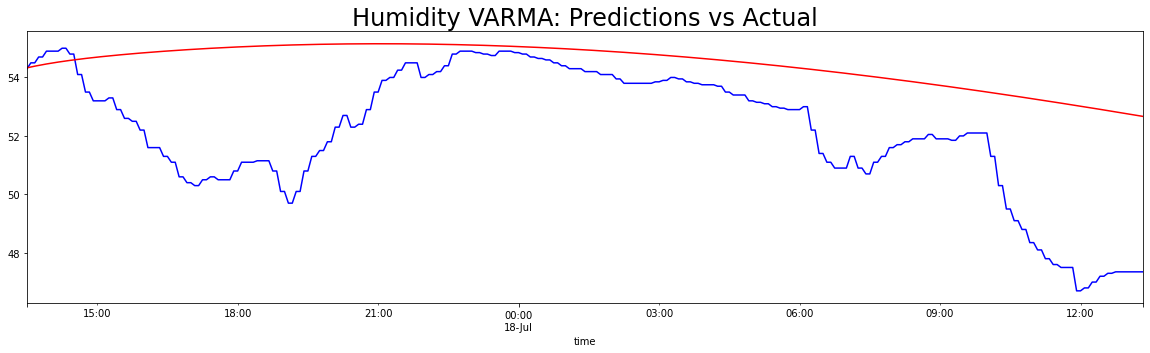
\includegraphics[width=12cm]{img/varmaHum.png} \label{fig:varmaHum}}}%
    \qquad
    \subfloat[Predizioni VARMA per 24 ore sui valori di pressione]
    {{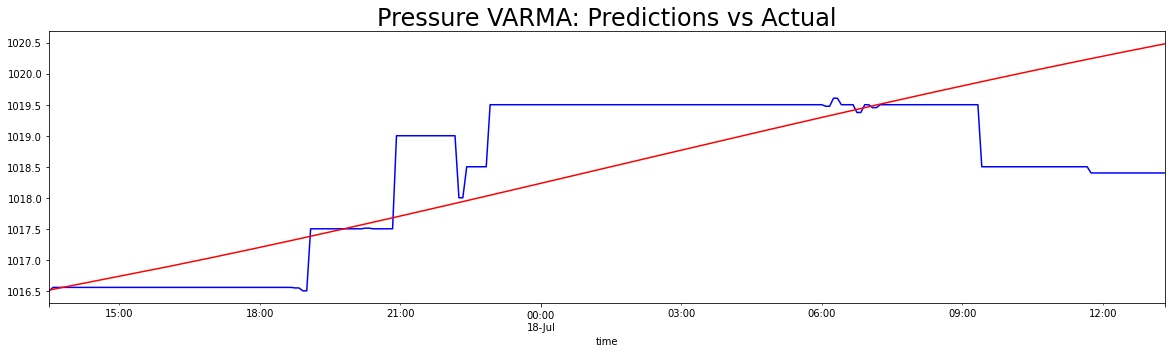
\includegraphics[width=12cm]{img/varmaPress.png}
    \label{fig:varmaPress}}}%
    \qquad
    \subfloat[Predizioni VARMA per 24 ore sui valori del numero di persone]
    {{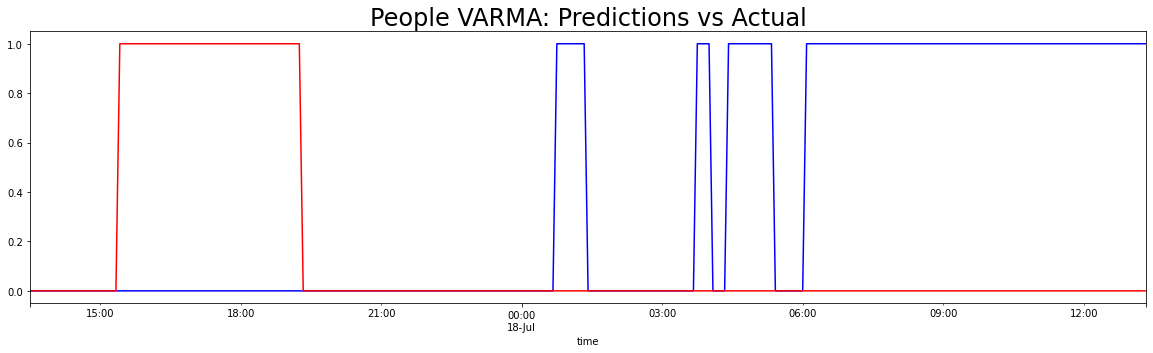
\includegraphics[width=12cm]{img/varmaPeople.png}
    \label{fig:varmaPeople}}}%
    \caption{Previsioni ottenute dal modello VARMA applicato ai dati di 11 giorni di temperatura, umidità e pressione per la previsione
    di una giornata. In rosso sono mostrati i valori predetti e in blu quelli attesi.}
    \label{fig:varma}
\end{figure}


\subsubsection{HWES}

Nei metodi come ARIMA viene sviluppato un modello in cui la previsione è una somma lineare ponderata delle osservazioni e errori recenti. I metodi di Exponential Smoothing sono simili in quanto la previsione è una somma ponderata delle osservazioni passate, ma il modello utilizza esplicitamente un peso in diminuzione esponenziale per le osservazioni passate. Il modello Holt-Winters Exponential Smoothing che è stato utilizzato permette supporto per il trend e la stagionalità \cite{hwes}.

Dato che il modello permette di settare la componente di stagionalità, si è considerata come stagionalità il corso di una giornata che, avendo aggregato i dati in modo da avere un punto ogni 5 minuti, è settata a 288 (12 punti/ora * 24 ore).
Il modello è allenato sui dati di 11 giorni e si è tentato di effettuare una previsione delle 24 ore successive.


\begin{table}
\centering
\begin{tabular}{l|r|r|r|r}
\multicolumn{5}{c}{{\cellcolor[rgb]{0.875,0.875,0.875}} Metodo HWES}                                                                                                                         \\ 
\hline
\rowcolor[rgb]{0.753,0.753,0.753}             & \multicolumn{2}{c|}{\textbf{ 2 h}}                                    & \multicolumn{2}{c}{\textbf{24 h }}                                    \\
\rowcolor[rgb]{0.753,0.753,0.753}             & \multicolumn{1}{c|}{\textbf{MAE}} & \multicolumn{1}{c|}{\textbf{MSE}} & \multicolumn{1}{c|}{\textbf{MAE}} & \multicolumn{1}{c}{\textbf{MSE}}  \\ 
\hline
\rowcolor[rgb]{0.875,0.875,0.875} temperatura & 0.248                             & 0.077                             & 1.689                             & 4.319                             \\
umidità                                       & 1.753                             & 4.247                             & 3.174                             & 13.600                            \\
\rowcolor[rgb]{0.875,0.875,0.875} pressione   & 0.164                             & 0.044                             & 0.638                             & 0.603                            
\end{tabular}
\caption{MAE e MSE ottenuto dalle predizioni di 2 ore e 24 ore sui dati di temperatura, umidità e pressione utilizzando il metodo HWES e un training set di 12 giorni}
\label{tab:hwes}
\end{table}


In Figura \ref{fig:hwes} si mostrano i risultati predetti da HWES (linea rossa) confrontati con i dati reali (linea blu) mentre in Tabella \ref{tab:hwes} sono elencati il valori MAE e MSE. Il modello è stato in grado, rispetto ai precedenti, di seguire meglio l'andamento della curva dei dati reali, ma i risultati in termini di MSE non sono ancora considerati soddisfacenti.


\begin{figure}
    \centering
    \subfloat[HWES per i valori di temperatura] {{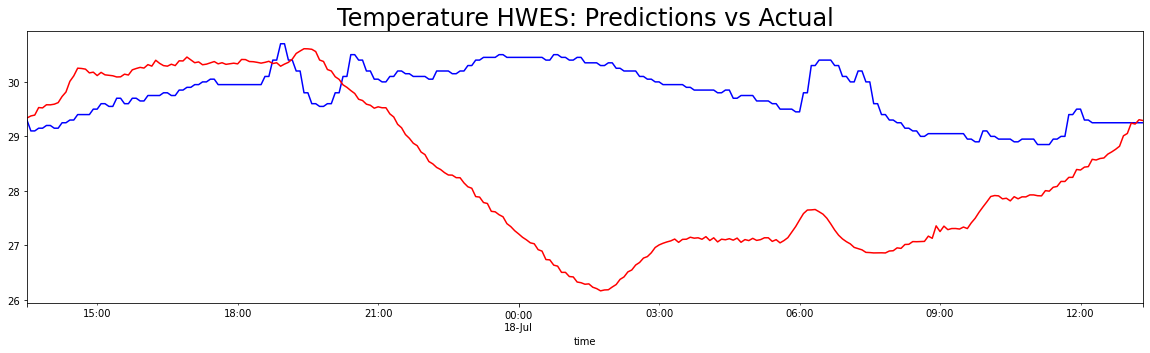
\includegraphics[width=10cm]{img/hwesTemp.png} \label{fig:hwesTemp}}}%
    \qquad
    \subfloat[HWES per i valori di umidità]
    {{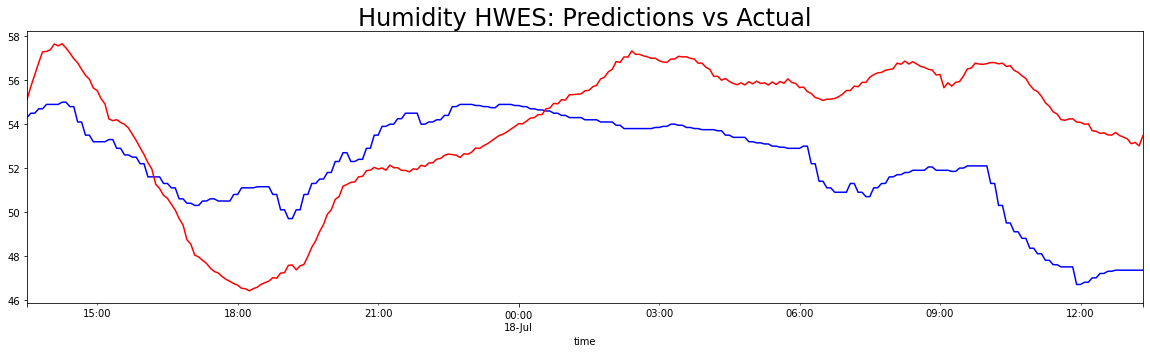
\includegraphics[width=10cm]{img/hwesHum.png} \label{fig:hwesHum}}}%
    \qquad
    \subfloat[HWES per i valori di umidità]
    {{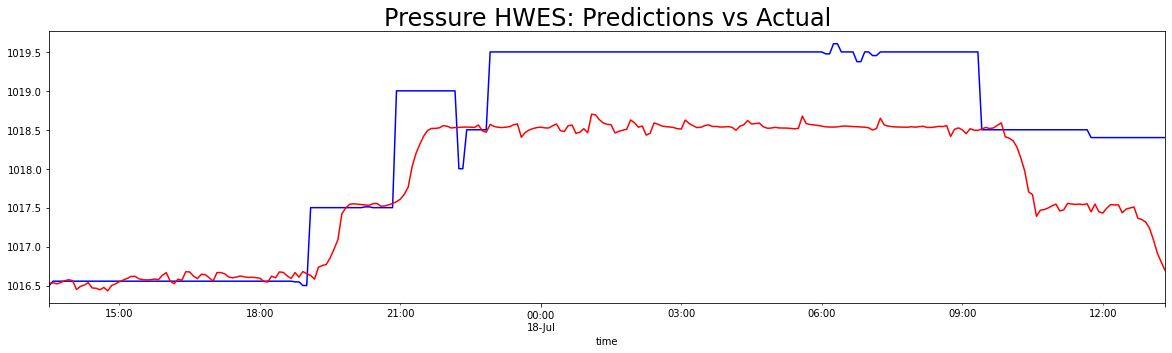
\includegraphics[width=10cm]{img/hwesPress.png} \label{fig:hwesPress}}}%
    \caption{Previsioni ottenute dal modello HWES applicato ai dati di temperatura, umidità e pressione per l'arco di una giornata}
    \label{fig:hwes}
\end{figure}


\subsubsection{LSTM\label{sec:lstm}} 
Il modello Long Short-Term Memory (LSTM) è un'archiettura Recurrent Neural Network (RNN) utilizzata nel campo del deep learning. Le LSTM sono RNN in grado di riconoscere schemi in delle sequenze di dati come le time-serie provenienti dai sensori.

Per preparare i dati per questo modello è stato necessario normalizzarli per inserirli in un intervallo $[0,1]$. Ci si è posti come obiettivo quello di predire i risultati per le 24 ore successive (24 ore * 12 punti/ora = 288 punti) basandosi sui valori del giorno precedente. Sia per il training set che per il validation set sono state create delle coppie in cui il primo elemento è la finestra temporale che precede il secondo e il il secondo elemento è la sequenza di valori da predire. Per rendere più efficace la predizione, la finestra temporale non comprende tutti i punti dell'intervallo, ma è stato campionato solamente un punto ogni quarto d'ora e quindi le finestre temporali saranno composte da $4*24=96$ punti.

Risulta quindi possibile costruire con l'utilizzo delle librerie di tensorflow il modello di una rete neurale a tre livelli composta da due LSTM e un Dense layer finale.
In un secondo momento è stato fatto quindi fitting del modello utilizzando 30 epoch. 

Per quanto riguarda la previsione del numero di persone dall'interno della stanza, è stato usata una RRN a 3 livelli come quella presentata sopra, ma è stata adattata utilizzando come funzione di attivazione sigmoid che risulta molto efficace nella predizione di valori di probabilità e che quindi ci permettesse di ottenere un livello di probabilità sulla presenza o meno della persona all'interno dell'ambiente. Infine i valori ottenuti sono stati arrotondati per ottenere un valore binario.

Risulta semplice anche valutare il MSE del modello e salvarlo per poterlo utilizzare in un servizio di forecasting. 
In Tabella \ref{tab:lstm} è possibile vedere gli errori MAE e MSE ottenuti dal modello per una previsione di 2 e 24 ore e con una history di un giorno e di due giorni.

I modelli risultano meno efficaci rispetto ad altri in termini di MAE e MSE, ma si è tenuto in considerazione il fatto che, mentre gli altri modelli devo essere allenati ogni volta, questa rete può essere allenata meno spesso, per esempio una volta ogni 2/3 giorni. Inoltre, gli altri modelli hanno bisogno di dati di almeno 10 giorni e quindi, per ogni predizione, sarebbe necessario effettuare una richiesta di molti dati a InfluxDB. Questo modello invece permette di fornire risultati affidabili anche con una storia molto più breve e questo permette di effettuare query a Influx che richiedano meno tempo e un minore spostamento di dati.
Infine si ritiene che, con l'aggiunta di nuovi dati, il modello LSTM possa diventare sempre più accurato nella previsione dei valori futuri.

Analizzando i risultati ottenuti dall'analisi dei modelli si è deciso quindi di utilizzare LSTM come modello per il servizio di forecasting facendo previsioni di 2 ore nel futuro.


\begin{table}
\centering
\begin{tabular}{l|r|r|r|r|r|r}
\multicolumn{7}{c}{{\cellcolor[rgb]{0.875,0.875,0.875}} Metodo LSTM}                                                                                                                                                                              \\ 
\hline
\rowcolor[rgb]{0.753,0.753,0.753}           & \multicolumn{4}{c|}{\textbf{ 1 day of history~ } }                                                                                            & \multicolumn{2}{c}{ \textbf{2 days of history}}              \\ 
\hline
\rowcolor[rgb]{0.875,0.875,0.875}           & \multicolumn{2}{c|}{2h prevision}                                     & \multicolumn{2}{c|}{24h prevision }                                   & \multicolumn{2}{c}{ 2h prevision}                   \\ 
\hline
\rowcolor[rgb]{0.753,0.753,0.753}           & \multicolumn{1}{c|}{\textbf{MAE}} & \multicolumn{1}{c|}{\textbf{MSE}} & \multicolumn{1}{c|}{\textbf{MAE}} & \multicolumn{1}{c|}{\textbf{MSE}} & \multicolumn{1}{c|}{\textbf{MAE}} & \multicolumn{1}{c}{\textbf{MSE}}  \\ 
\hline
temperatura                                 & 1.144                             & 1.957                             & 2.109                             & 7.238                             & 1.128                    & 2.156                    \\
\rowcolor[rgb]{0.875,0.875,0.875} umidità   & 3.168                             & 16.709                            & 7.244                             & 74.065                            & 2.413                    & 15.157                   \\
pressione                                   & 1.879                             & 4.427                             & 2.406                             & 7.715                             & 1.765                    & 3.780                    \\
\rowcolor[rgb]{0.875,0.875,0.875} n persone & 0.340                             & 0.185                             & 0.452                             & 0.25                              & 0.367                    & 0.187                   
\end{tabular}
\caption{MAE e MSE ottenuti dalle predizioni di un 2 ore e 24 ore con una history di 1 giorno e di 2 ore con una history di due giorni utilizzando il metodo LSTM e un traing set di 9 giorni}
\label{tab:lstm}
\end{table}


\begin{figure}
    \centering
    \subfloat[Predizioni LSTM per 24 ore sui valori di temperature]
    {{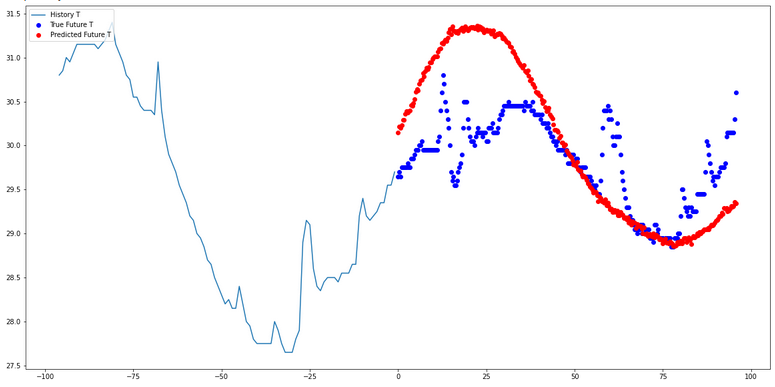
\includegraphics[width=7.5cm]{img/lstmTemp.png}}}%
    \qquad
    \subfloat[Predizioni LSTM per 24 ore sui valori di umidità]
    {{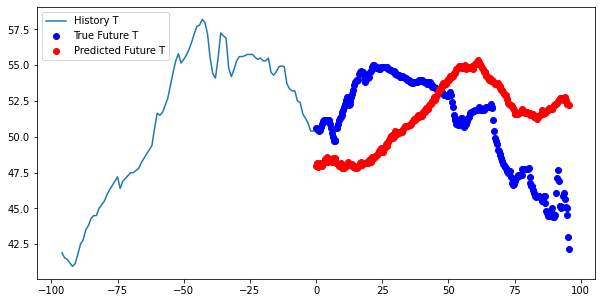
\includegraphics[width=7.5cm]{img/lstmHum.png}}}%
    \qquad
    \subfloat[Predizioni LSTM per 24 ore sui valori di pressione]
    {{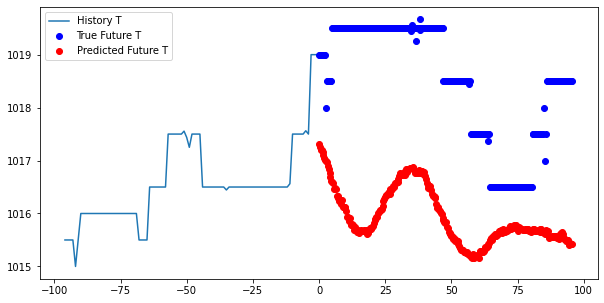
\includegraphics[width=7.5cm]{img/lstmPress.png}}}%
    \qquad
    \subfloat[Predizioni LSTM per 24 ore sui valori del numero di persone]
    {{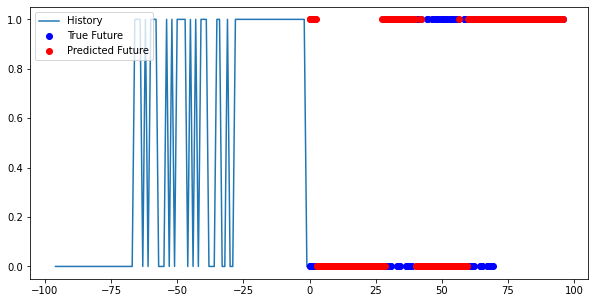
\includegraphics[width=7.5cm]{img/lstmPeople.png}}}%
    \caption{Previsioni ottenute dal modello LSTM per 24 ore con uno storico di 24 ore per i valori di temperatura, umidità, pressione e numero di persone. I punti in rosso rappresentano i valori predetti mentre quelli in blu i valori attesi, in azzuro è rappresentata la finestra temporale utilizzata per predirre i nuovi valori}
    \label{fig:lstm}
\end{figure}

\subsection{Servizio di forecasting}

\subsubsection{Calcolo della previsione}
Utilizzando Python è stato costruito un servizio che si occupi di ricevere richieste di previsioni e, sfruttando i modelli per il forecasting di temperatura, pressione, umidità e numero di persone, di calcolare la previsione per ognuna delle misurazioni per le due ore a seguire. Tale servizio utilizza come modelli i modelli ottenuti dalla rete neurale LSTM.

Il servizio deve essere in grado interrogare InfluxDB per ottenere i dati delle diverse misurazione delle ultime 24 ore. I dati ottenuti vengono normalizzati e forniti come input ai modelli salvati. Ottenuta una previsione per i valori di temperatura, umidità, pressione e numero di persone, viene creata una struttura json che è mandata in risposta alla richiesta di previsione.


\subsubsection{Richiesta della previsione}
Utilizzando Typescript è stato costruito un servizio, WriterService, che si occupa a intervalli regolari di:
\begin{enumerate}
    \item Eseguire un richiesta di previsione verso il ForecastingService;
    \item Elaborare la risposta ottenuta e creare un nuovo punto per ogni previsione ottenuta;
    \item Caricare su InfluxDB tutti i punti contenenti le previsioni.
\end{enumerate}

Dato che InfluxDB supporta caricamenti batch fino a 5000 punti, le scritture vengono effettuate con un unica chiamata al fine di non saturare di richieste il database.

\subsection{Visualizzazione dei dati}
La visualizzazione dei dati avviene attraverso le dashboard di Grafana. In Figura \ref{fig:grafana} sono mostrati i grafici su Grafana ottenuti interrogando InfluxDB per avere i dati, aggregati ogni 30 minuti, di temperatura, umidità, pressione e numero di persone.

\begin{figure}
    \centering
    {{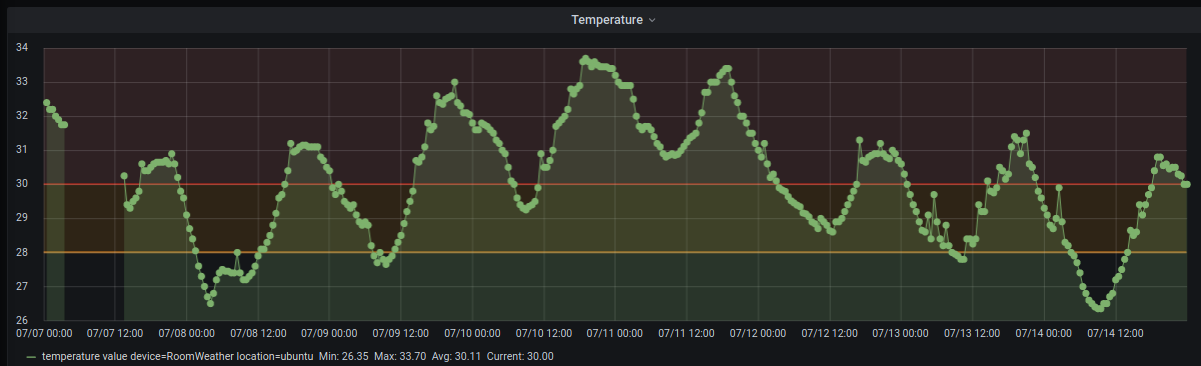
\includegraphics[width=13cm]{img/grafanaTemp.png}}}%
    \bigskip
    \qquad
    {{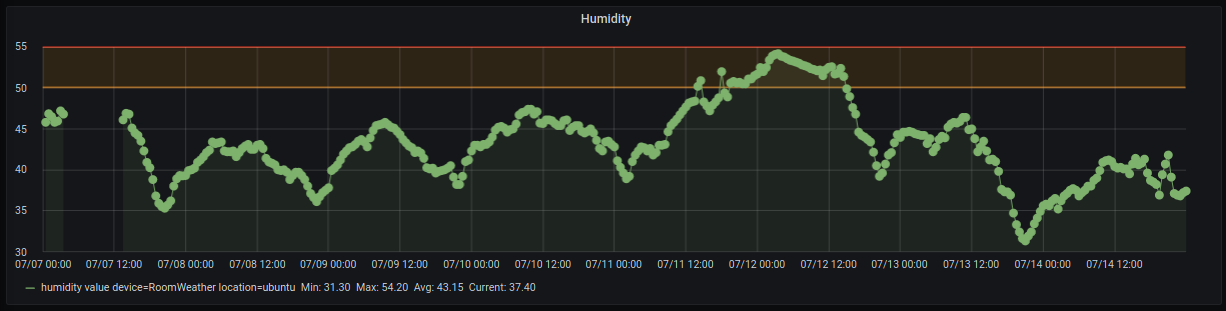
\includegraphics[width=13cm]{img/grafanaHumidity.png}}}%
    \bigskip
    \qquad
    {{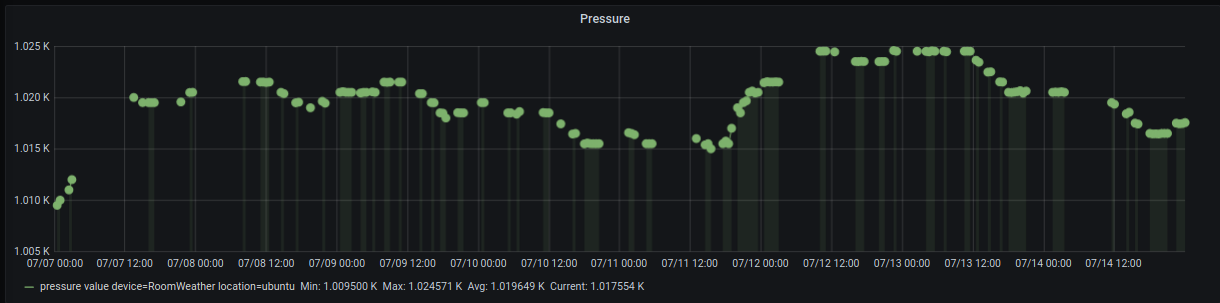
\includegraphics[width=13cm]{img/grafanaPressure.png}}}%
    \bigskip
    \qquad
    {{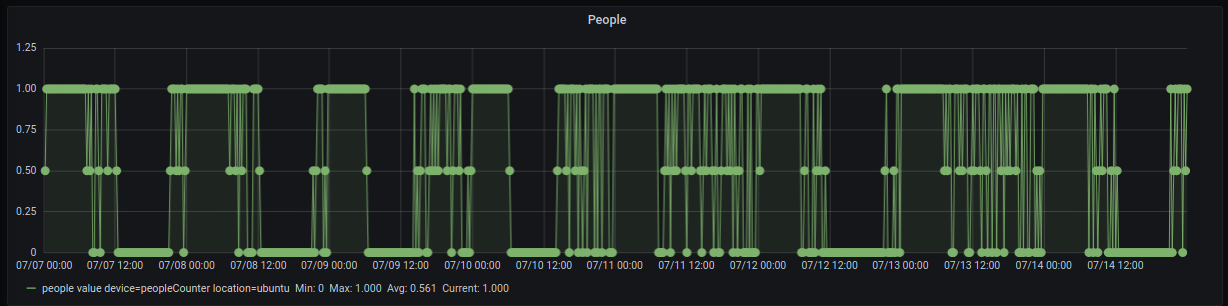
\includegraphics[width=13cm]{img/grafanaPeople.png}}}%
    \caption{Visualizzazione attraverso Grafana delle dashboard di temperatura, umidità, pressione e numero di persone}
    \label{fig:grafana}
\end{figure}


\subsection{Servizio di alerting}
Utilizzando gli alert di InfluxDB è stato possibile costruire un servizio di alerting che permette di notificare l'utente tramite un bot di Telegram. 

Su InfluxDB sono stati settati tramite script due alert che consentono di ricevere un avviso tramite il bot di Telegram quando i valori di temperatura e umidità superano una certa soglia preimpostata.


\subsection{Script ausiliari}
\begin{itemize}
    \item Uno script che permette di creare un ambiente completo su InfluxDB con organizzazione, utente, buket e relativa autorizzazione;
    \item Uno script per la creazione degli alert su InfluxDB.
\end{itemize}



\begin{figure}
    \centering
    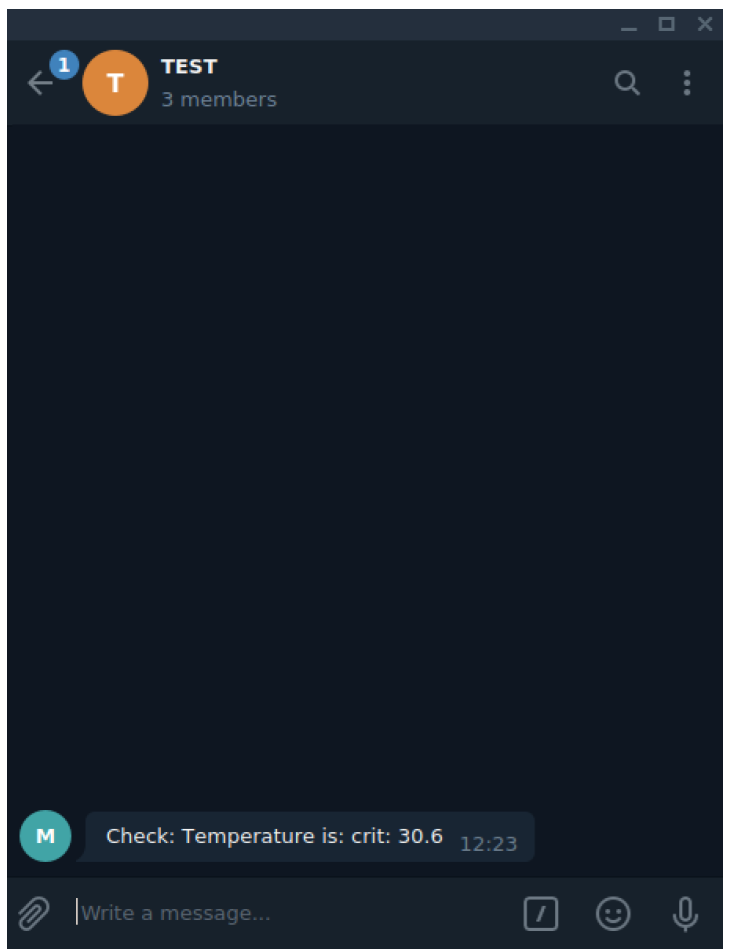
\includegraphics[width=5cm]{img/AlertBot.png}
    \caption{Bot di Telegram per la notifica di situazioni di "pericolo" nell'ambiente}
    \label{fig:influxForecast}
\end{figure}

\section{Risultati \label{section:risultati}}
Entrambe le Wot Thing costruite, RoomWeather e PeopleCounter, si sono dimostrate affidabili in fase di prototipazione e sono quindi state installate in una stanza per poter raccogliere i dati dell'ambiente. 
 
La thing PeopleCounter è stata testata anche in contesti di luci diverse per valutare se l'influenza di luci esterne potesse creare problemi nel conteggio dei passaggi, dato che in un primo momento le fotoresistenze erano influenzate da altre luci molto forti si è deciso di applicare un filtro per la luce rossa al prototipo. Questa miglioria ha permesso di rendere il servizio efficiente in diversi contesti luminosi.

La problematica principale riscontrata consiste nel numero limitato di misurazioni che sono state prodotte, questo ha causato un'efficacia limitata nelle previsioni attraverso i metodi di forecasting.

Per quanto riguarda il modello di forecasting sui dati è stato selezionato LSTM che, nonostante non presentasse il miglior MSE, presenta grandi vantaggi in termini di efficienza nel momento in cui devono essere svolte le previsioni. I dettagli sull'analisi dell'errore calcolato per LSTM possono essere trovati nella Sezione \ref{sec:lstm}.





\section{Conclusione e sviluppi futuri}
Si ritiene che il sistema possa essere efficacemente utilizzato in contesti reali di monitoraggio di ambienti fornendo la possibilità di costruire a basso costo un sistema efficace e senza un eccessivo dispendio energetico. L'utilizzo di Docker e Docker Compose ha reso il sistema costruito semplice da riprodurre e aggiornare, in particolare è possibile sostituire il servizio di forecasting o aggiornare i modelli che utilizza semplicemente sostituendo un container. 

Ci si propone di migliorare la rete neurale che fornisce la previsione dei risultati anche se ci si aspetta che un insieme di dati più grandi su cui fare training possa essere sufficiente per ottenere previsioni più efficaci. Inoltre si propone come sviluppo futuro quello di arricchire il servizio di forecasting con la possibilità di caricare la nuova rete LSTM allenata.





\bibliographystyle{plain}
\bibliography{references}
\end{document}
